\documentclass[11pt,a4paper]{article}
\usepackage[T1]{fontenc}
\usepackage[utf8]{inputenc}
\usepackage{lmodern}
\usepackage[margin=27mm]{geometry}
\usepackage{amsmath,amssymb,amsthm,mathtools}
\usepackage{booktabs,array,tabularx}
\usepackage{microtype}
\usepackage{xcolor}
\usepackage{tikz}
\usetikzlibrary{arrows.meta,calc,positioning}
\usepackage[font=small,labelfont=bf]{caption}
\usepackage{enumitem}
\setlist{topsep=3pt,itemsep=2pt}
\usepackage[colorlinks=true,linkcolor=blue!50!black,citecolor=blue!50!black,urlcolor=blue!50!black]{hyperref}
\usepackage[nameinlink,capitalise]{cleveref}

\usepackage{aliascnt}
\newtheorem{theorem}{Theorem}[section]
\newcommand{\sharedthm}[3][plain]{%
  \newaliascnt{#2}{theorem}%
  \theoremstyle{#1}\newtheorem{#2}[#2]{#3}\aliascntresetthe{#2}%
  \crefname{#2}{#3}{#3s}}
\sharedthm{lemma}{Lemma}
\sharedthm{corollary}{Corollary}
\sharedthm{proposition}{Proposition}
\sharedthm{conjecture}{Conjecture}
\theoremstyle{plain}
\crefname{corollary}{Corollary}{Corollaries}
\newtheorem*{dgconj}{Conjecture 1 of Dorsman and Gardner}
\sharedthm[definition]{definition}{Definition}
\sharedthm[definition]{example}{Example}
\sharedthm[remark]{remark}{Remark}
\theoremstyle{plain}
\crefname{corollary}{Corollary}{Corollaries}

\newcommand{\rev}{\operatorname{rev}}
\newcommand{\W}{\mathsf{W}}
\newcommand{\Or}{\mathsf{A}}
\newcommand{\dep}{\operatorname{dep}}
\newcommand{\up}{\operatorname{up}}
\newcommand{\Nout}{N^{+}}
\newcommand{\Nin}{N^{-}}
\newcommand{\Bal}{\mathcal{B}}
\newcommand{\Obal}{\mathcal{O}}
\newcommand{\Pat}{\mathcal{P}}
\newcommand{\K}{\mathcal{K}}
\newcommand{\G}{\Gamma}
\newcommand{\Sg}{\Sigma}
\newcommand{\empt}{\varnothing}
\newcommand{\what}[1]{\par\smallskip\noindent\textit{What this means.} #1\par\smallskip}

\tikzset{
  vtx/.style={circle,draw=black!70,fill=white,inner sep=0pt,minimum size=5.6mm,font=\small},
  src/.style={vtx,fill=black!12},
  snk/.style={vtx,fill=black!12,double,double distance=0.6pt},
  arc/.style={-{Stealth[length=2.4mm]},thick,black!70,shorten >=0.5pt,shorten <=0.5pt},
  hot/.style={-{Stealth[length=2.6mm]},very thick,orange!80!black,shorten >=0.5pt,shorten <=0.5pt},
  longp/.style={-{Stealth[length=2.4mm]},very thick,blue!60!black,shorten >=0.5pt,shorten <=0.5pt}
}

\title{Bounded swaps in pass-and-swap queues:\\
counterexamples to a conjecture of Dorsman and Gardner,\\
and a proof for bipartite swapping graphs\\ with odd caps under positive service rates}
\author{Anonymous}
\date{20 October 2026}

\begin{document}
\maketitle

\begin{abstract}
Dorsman and Gardner (2024) studied closed tandems of two pass-and-swap queues in which a service completion may trigger at most $w$ swaps. The relative positions of the jobs define an acyclic orientation of the swapping graph. They proved product-form stationary laws when this orientation has no directed path longer than $w$ edges, and conjectured that, when the swapping graph is $(w+1)$-colourable, every state with a longer directed path (a state of \emph{excessive height}) is transient. The conjecture would have implied that every recurrent class lies in a single orientation of height at most $w$ and carries the corresponding product-form law.

We show that the conjecture fails for every $w\ge2$, and we locate where it fails and where it holds. Below, ``positive rates'' means that every position of every queue is served at a positive rate. On the cycle $C_n$ with positive rates, a recurrent class of excessive height exists if and only if $n\equiv1\pmod{2w}$, and it is then the unique such class; for $n=2w+1$ it has $(2w+2)!/(w!)^2$ states, and the class is closed for every admissible rate function. So, for $w\ge2$ (where every cycle satisfies the colouring hypothesis), the conjecture fails on $C_n$ exactly when $n\equiv1\pmod{2w}$. Two odd cycles joined by a path give a family of counterexamples that are not cycles. An exact census of all connected graphs on at most seven vertices finds 1355 violating pairs (graph, cap), none of them bipartite and none at $w=1$. Conversely, for bipartite swapping graphs and odd $w$, the conjecture holds under positive rates. Computation supports the same statement for every $w$ on all bipartite graphs with at most nine vertices. The proofs rest on two tools: a description of the orientation changes that a capped service can cause (all of them, under positive rates), and the identification of service with truncated promotion on linear extensions. On the high recurrent class of $C_{2w+1}$, homogeneous rates give an explicit product-form law. For additive per-job rates and every $w\ge2$, scaling the original product weights on this class by one constant per orientation gives a stationary law only when the rates are constant within each queue (the two queues may differ); the low classes keep the ordinary product form for any rates. All finite claims are certified by exact, replayable verifiers. This manuscript has not been peer reviewed.
\end{abstract}

\tableofcontents

\section{Introduction}\label{sec:intro}

\subsection{Pass-and-swap queues in brief}

Many service systems match jobs with compatible resources: servers in a cluster, donors and patients, drivers and riders. A recurring difficulty in such models is that their stationary behaviour rarely has a closed form. One family where it does is that of order-independent queues~\cite{BKK1995,Krz2011}, which contains multi-server systems with job--server compatibilities under first-come-first-served service~\cite{VAW2012,GR2020}, and token-based central queues~\cite{ABDV2022}, and it is closely related to insensitive allocations such as balanced fairness~\cite{BP2003}. Their stationary distribution has a \emph{product form}: it is a product of simple factors, one per position in the queue.

Comte and Dorsman~\cite{CD2021} extended this family with \emph{pass-and-swap} queues. Jobs belong to classes, and a \emph{swapping graph} on the classes says which jobs may exchange places. When a job completes service it does not necessarily leave. Instead it scans the jobs behind it, takes the place of the first one it may swap with, and that job, in turn, scans further back. The last job in this chain leaves the queue. Comte and Dorsman proved that the product form survives this extra routing. Dorsman and Gardner~\cite{DG2024} then asked what happens when at most $w$ swaps are allowed per service completion: the $w$-th displaced job must leave even if it could swap further.

\paragraph{Why caps on swaps.} The motivation for caps comes from redundancy scheduling. In the redundancy-$d$ model each job is sent to $d$ servers and is cancelled everywhere when one copy completes~\cite{GZDHHS2016,GHSVZ2017,ABV2018}. Its stationary law is known under first-come-first-served service, but not under random order of service; Anton and Gardner conjectured that the two disciplines give the same law~\cite{AG2023}, and Gast and Van Houdt gave numerical evidence that they do not~\cite{GVH2024}. Dorsman and Gardner observed that random order of service can be written as a pass-and-swap queue with a random, state-dependent cap, so a proof that caps preserve the stationary law would settle this question~\cite[Section~5]{DG2024}. As a first step they studied fixed caps.

\paragraph{Placement orientations.} In a closed tandem of two pass-and-swap queues, jobs circulate between an upper and a lower queue. Reading the upper queue from head to tail and then the lower queue from tail to head gives a word on the jobs, the \emph{global word}. Orienting every edge of the swapping graph from its earlier to its later endpoint in this word gives an acyclic orientation, the \emph{placement orientation} (Dorsman and Gardner's \emph{placement order}). Without a cap, no service completion ever changes it~\cite{CD2021}; so the state space splits into closed pieces, one per orientation, and each piece carries the product-form law.

A cap can change the orientation, but only when it actually stops a swap chain. Every swap chain follows a directed path of the orientation. So, if the longest directed path has at most $w$ edges, the cap never binds, the orientation never changes, and the uncapped product form applies~\cite[Theorem~7]{DG2024}.

\subsection{The conjecture and why it mattered}

Call an orientation \emph{low} if its longest directed path has at most $w$ edges and \emph{high} otherwise. Low orientations exist exactly when the swapping graph can be properly coloured with $w+1$ colours (the Gallai--Roy theorem~\cite{Roy1967}; see~\cite[Lemma~3]{DG2024}). Dorsman and Gardner conjectured that, under this colouring condition, high orientations cannot persist. The conjecture is quoted in full in \cref{sec:conj}. In words: if the swapping graph is $(w+1)$-partite, every state with a high placement orientation is transient. They reported that ``extensive numerical experiments'' supported it, and drew the consequence that, under the colouring condition, ``the stationary distribution of the closed tandem network is always of product form''~\cite[Section~5.2.2]{DG2024}. Since the chain is not irreducible, we read this classwise: every recurrent class would lie in $\Sg_A$ for a single low orientation $A$ and carry the corresponding product-form law, so that every stationary distribution would be a mixture of these laws. In their appendix they also remarked that a proof ``would be easy if all jobs in the system were allocated a positive service rate at all times''~\cite[Appendix~C.2]{DG2024}.

\subsection{Contributions}\label{sec:contrib}

Throughout, there is one job per class (the general case reduces to this one, \cref{prop:multiplicity}), the swapping graph is simple, and the cap $w$ is the same in both queues.

\begin{enumerate}[label=\textbf{C\arabic*.},leftmargin=*]
\item \textbf{Tools} (\cref{sec:tools}). \Cref{lem:moves} describes the orientation changes a capped service can cause; under positive rates (PR) the list is exact. With (PR), it reduces the recurrence question to a finite directed graph on orientations (\cref{cor:reduction}). \Cref{prop:promotion} identifies pass-and-swap service with Sch\"utzenberger promotion on linear extensions~\cite{Sch1972,Sta2009,AKS2014}, truncated by the cap.
\item \textbf{The basic counterexample} (\cref{sec:oddcycle}). For every $w\ge2$, the balanced states of $C_{2w+1}$ form a closed set of height $w+1$, which under (PR) is a single recurrent class, with $(2w+2)!/(w!)^2$ states (\cref{thm:balanced}). Conjecture~1 is therefore false for every $w\ge2$ (\cref{cor:false}). Closure of the class holds for every admissible service-rate function, including service at the head of each queue only (\cref{rem:anyrates}).
\item \textbf{All cycles} (\cref{sec:cycles}). Under (PR), $C_n$ has a recurrent class of excessive height if and only if $n\equiv1\pmod{2w}$, and it is then the unique class of excessive height (\cref{thm:cycles}); without (PR) the set is shown to be closed. Among cycles satisfying the hypothesis $\chi(C_n)\le w+1$, that is for $w\ge2$, the conjecture under (PR) therefore fails exactly when $n\equiv1\pmod{2w}$; for example $C_9$ with $w=2$ is a counterexample whose odd girth exceeds $2w+1$.
\item \textbf{Beyond cycles} (\cref{sec:beyond}). Two odd cycles joined by a path form a counterexample at one explicit cap (\cref{thm:twocycles}). An exact census of all connected graphs with at most seven vertices (\cref{tab:census}) finds, under (PR), that violations are common for $w\ge3$, absent for the bipartite graphs in the census and absent at $w=1$. Several jobs per class reduce to one job per class (\cref{prop:multiplicity}). Extra jobs remove the counterexamples on the cycles we checked, but not in general (\cref{tab:mult}).
\item \textbf{Where the conjecture holds} (\cref{sec:bipartite}). For a bipartite swapping graph, an odd cap and positive service rates (PR), every state of excessive height is transient (\cref{thm:bipartite}). This includes the setting of Dorsman and Gardner's worked examples for the conjecture: paths with $w=1$. We conjecture the same for even caps (\cref{conj:bipartite}), supported by exact computation on all bipartite graphs with at most nine vertices.
\item \textbf{Stationary laws} (\cref{sec:stationary}). On the balanced class, homogeneous rates give a uniform global word independent of a binomial split. This law also satisfies Dorsman and Gardner's partial-balance equations (\cref{thm:homog,prop:partial}). For additive per-job rates and every $w\ge2$, multiplying the original product weights on $\Bal_w$ by one positive constant per orientation gives a stationary law only if the rates are constant within each queue (\cref{thm:hetero}); the two queues may have different constants, and the low classes keep the ordinary product form for any rates. On $C_5$ the orientation-matched approximation is within total variation $2\times10^{-3}$ of the true law in our computations, and the long-run behaviour depends on the initial state (\cref{tab:deviation}).
\end{enumerate}

All finite statements are checked by exact, deterministic, standard-library programs (\cref{sec:data}). The proofs do not depend on these programs.

\subsection{A first example: the five-cycle with cap two}\label{sec:firstexample}

Take five jobs $0,\dots,4$ whose swapping graph is the cycle $C_5$ (job $i$ may swap with $i\pm1 \bmod 5$), cap $w=2$, and all jobs in the upper queue in the order $(0,1,2,4,3)$. The global word is $01243$. The placement orientation therefore has the single source $0$ and the single sink $3$, joined by the directed paths $0\to1\to2\to3$ (three edges) and $0\to4\to3$ (two edges); see \cref{fig:c5}, left.

Suppose the head job $0$ completes service. It scans backwards, finds its neighbour $1$ and takes its place; job $1$ finds $2$ and takes its place. That is two swaps, so the cap stops the chain: job $2$ must leave, although it could have swapped with $3$. The new state has upper queue $(0,1,4,3)$ and lower queue $(2)$, with global word $01432$. Exactly one edge has changed direction: $2\to3$ became $3\to2$. The sink has moved from $3$ to $2$, and the two paths from source to sink now have two and three edges (\cref{fig:c5}, right).

Thus the cap moved the sink, but the longest path still has three edges. \Cref{thm:balanced} shows that this always happens. Every orientation with one source and one sink joined by paths of two and three edges is mapped by every possible service completion to another orientation of the same kind. With positive service rates, the $180$ states with such orientations form one recurrent class. A direct enumeration of all $720$ states confirms this. There are ten closed classes of $48$ states with longest path two and the class of $180$ states with longest path three. The remaining $60$ states are transient. Since $C_5$ is $3$-colourable and $3=w+1$, the $180$ recurrent states of height $3>w$ contradict the conjecture.

\begin{figure}[t]
\centering
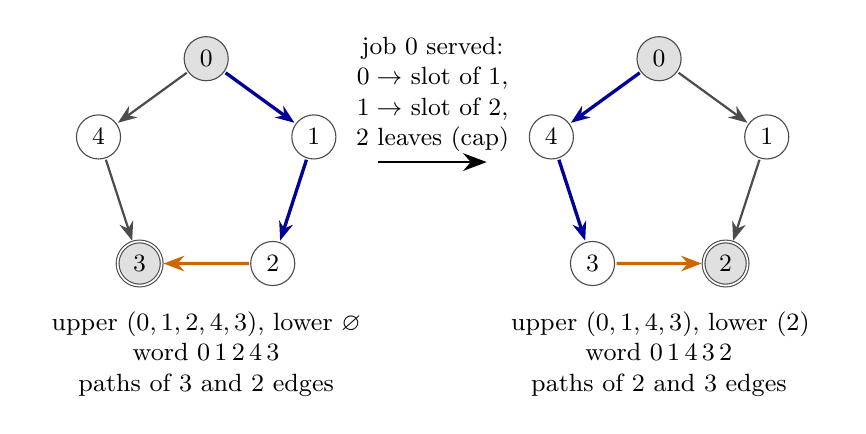
\begin{tikzpicture}[scale=1.25]
\foreach \side/\dx in {L/0,R/4.6}{
  \foreach \v in {0,...,4}{ \coordinate (\side\v) at ($(\dx,0)+(90-72*\v:1.15)$); }
}
\node[src] (a0) at (L0) {0}; \node[vtx] (a1) at (L1) {1}; \node[vtx] (a2) at (L2) {2};
\node[snk] (a3) at (L3) {3}; \node[vtx] (a4) at (L4) {4};
\draw[longp] (a0)--(a1); \draw[longp] (a1)--(a2); \draw[hot] (a2)--(a3);
\draw[arc] (a4)--(a3); \draw[arc] (a0)--(a4);
\node[font=\small,align=center,text width=4.3cm] at (0,-1.85) {upper $(0,1,2,4,3)$, lower $\empt$\\ word $0\,1\,2\,4\,3$\\ paths of $3$ and $2$ edges};
\node[src] (b0) at (R0) {0}; \node[vtx] (b1) at (R1) {1}; \node[snk] (b2) at (R2) {2};
\node[vtx] (b3) at (R3) {3}; \node[vtx] (b4) at (R4) {4};
\draw[arc] (b0)--(b1); \draw[arc] (b1)--(b2); \draw[hot] (b3)--(b2);
\draw[longp] (b4)--(b3); \draw[longp] (b0)--(b4);
\node[font=\small,align=center,text width=4.3cm] at (4.6,-1.85) {upper $(0,1,4,3)$, lower $(2)$\\ word $0\,1\,4\,3\,2$\\ paths of $2$ and $3$ edges};
\draw[-{Stealth[length=3mm]},thick] (1.75,0.1) -- node[above,font=\small,align=center]{job $0$ served:\\ $0\to$ slot of $1$,\\ $1\to$ slot of $2$,\\ $2$ leaves (cap)} (2.85,0.1);
\end{tikzpicture}
\caption{The first example (\cref{sec:firstexample}). Shaded vertex: source; double circle: sink. The thick blue path is the longest directed path. Only the orange edge $\{2,3\}$ is reversed by the capped service. The sink moves from $3$ to $2$, and the source--sink path lengths $\{2,3\}$ are preserved.}
\label{fig:c5}
\end{figure}

\subsection{Related work}

Order-independent queues go back to Berezner, Kriel and Krzesinski~\cite{BKK1995}; see Krzesinski's survey~\cite{Krz2011}. Product forms for first-come-first-served systems with job--server compatibilities are surveyed by Gardner and Righter~\cite{GR2020}. They include redundancy models~\cite{GZDHHS2016,GHSVZ2017,ABV2018} and the token-based central queue~\cite{ABDV2022}. Pass-and-swap queues~\cite{CD2021} cover, among others, stochastic matching models with order-independent loss~\cite{Com2022}. The bounded-swap variant and Conjecture~1 are due to Dorsman and Gardner~\cite{DG2024}, who also proved the product form on the low orientations (their Theorem~7). The colouring condition is the Gallai--Hasse--Roy--Vitaver duality between chromatic number and longest paths in acyclic orientations~\cite{Roy1967}.

On the combinatorial side, the operators we meet are promotion and its extensions on linear extensions~\cite{Sch1972,Sta2009,AKS2014}. Ayyer, Klee and Schilling~\cite{AKS2014} studied Markov chains driven by extended promotion on the linear extensions of a \emph{fixed} poset. Their stationary laws include uniform ones, obtained from bijectivity, and products of reciprocal prefix sums, the same factors as in the queueing weights. The capped chains here move between \emph{different} posets, so their results do not apply directly, but they explain where the familiar factors come from. Changing an acyclic orientation by reversing edges at a vertex is classical: Pretzel's source-to-sink pushes~\cite{Pre1986}, Propp's lattice structure on orientations~\cite{Pro2025}, Defant's toric promotion~\cite{Def2023} and the toric posets of Develin, Macauley and Reiner~\cite{DMR2016}. The binding moves of \cref{lem:moves} are of a different kind: they reverse only some of the edges at a vertex that is neither a source nor a sink. On cycles they act like a ``rotation'' of runs; the head map of \cref{sec:stationary} is a cyclic rotation of binary words, a standard example of cyclic sieving~\cite{RSW2004}.

\subsection{Roadmap}

\Cref{sec:model} fixes the model and notation (\cref{tab:notation}), quotes the conjecture with the source's definitions and reconciles conventions. \Cref{sec:tools} proves the tools used everywhere else. \Cref{sec:oddcycle} gives the basic counterexample in detail, \cref{sec:cycles} classifies cycles, and \cref{sec:beyond} treats other graphs and several jobs per class. \Cref{sec:bipartite} proves the positive result for bipartite graphs with odd caps. \Cref{sec:stationary} studies stationary laws on the balanced class. \Cref{sec:discussion} summarises what survives of the conjecture and lists open problems. \Cref{sec:data} describes the verification programs.

\section{Model, notation and the conjecture}\label{sec:model}

\subsection{States, words and orientations}

Let $G=(V,E)$ be a finite simple graph with $n=|V|$ vertices, the \emph{swapping graph}. There is one job per vertex, and we identify jobs with vertices. A \emph{state} is a pair $(c;d)$ of disjoint sequences whose union is $V$: the upper queue $c=(c_1,\dots,c_k)$ and the lower queue $d=(d_1,\dots,d_{n-k})$, each listed from head to tail. There are $(n+1)!$ states.

\begin{definition}[Global word, placement orientation, height]\label{def:orient}
The \emph{global word} of $(c;d)$ is $\W(c;d)=c_1\cdots c_k\,d_{n-k}\cdots d_1$, the upper queue followed by the reversed lower queue. Its \emph{placement orientation} $\Or(c;d)$ orients each edge of $G$ from its earlier to its later endpoint in $\W(c;d)$. For an acyclic orientation $A$ we write $P_A$ for the partial order it generates (so $u<v$ when $A$ has a directed path from $u$ to $v$), $\Sg_A$ for the set of states with $\Or(c;d)=A$, and $h(A)$ for the \emph{height}: the number of edges in a longest directed path of $A$. For a vertex $v$, $\dep_A(v)$ (the depth) and $\up_A(v)$ are the numbers of edges in a longest directed path ending, respectively starting, at $v$. $\Nout_A(v)$ and $\Nin_A(v)$ are the out- and in-neighbours of $v$. Given a cap $w$, an orientation is \emph{low} if $h(A)\le w$ and \emph{high} otherwise.
\end{definition}

The global word of a state is a linear extension of $P_{\Or(c;d)}$, and every linear extension together with every split point $k\in\{0,\dots,n\}$ gives exactly one state. Hence $|\Sg_A|=(n+1)\,e(A)$, where $e(A)$ is the number of linear extensions of $P_A$. A \emph{down-set} of $P_A$ is a set $D$ such that $v\in D$ and $u<v$ imply $u\in D$; up-sets are defined dually. The upper queue of a state of $\Sg_A$ is a down-set.

\subsection{The capped pass-and-swap transition and service rates}

\begin{definition}[Capped transition]\label{def:transition}
Fix a cap $w\ge1$. Suppose the job in position $p$ of the upper queue completes service. Remove it; it becomes the first \emph{carrier} $\gamma_0$. Starting just behind position $p$, scan towards the tail for the first job adjacent to the current carrier in $G$. If one is found, the carrier takes that job's position and the displaced job becomes the next carrier, and the scan continues strictly behind that position. Stop after $w$ such replacements, or earlier if no adjacent job remains behind. The final carrier joins the tail of the lower queue. Service in the lower queue is defined in the same way with the roles of the queues exchanged. The transition \emph{binds} the cap if the scan would have made more than $w$ replacements without the cap.
\end{definition}

A transition with exactly $w$ replacements need not bind. Without a cap ($w=\infty$) this is the pass-and-swap mechanism of~\cite{CD2021}; with a cap it is the mechanism of~\cite[Section~5]{DG2024}, in which ``the $w$-th job to be ejected from its original position must depart from the system''.

The service rates follow the order-independent model. The upper queue has a function $\mu$ on sets of jobs, invariant under reordering, with $\mu(\empt)=0$; the job in position $j$ of $c$ is served at rate $\Delta\mu(c_1,\dots,c_j)=\mu(c_1,\dots,c_j)-\mu(c_1,\dots,c_{j-1})\ge0$, and $\mu(i)>0$ for every single job $i$. The lower queue has an analogous function $\nu$. These conditions guarantee only that the head of a non-empty queue is served at a positive rate. Several results assume more:

\smallskip
\noindent\textbf{Positive rates (PR).} Every position of every non-empty queue is served at a positive rate.
\smallskip

\noindent The main example is the additive case $\mu(c)=\sum_{i\in c}\mu_i$ and $\nu(d)=\sum_{i\in d}\nu_i$ with positive $\mu_i,\nu_i$; the rate at a position is then that of the job occupying it. Homogeneous rates are $\mu_i\equiv\mu_0$ and $\nu_i\equiv\nu_0$. Which states are recurrent depends only on which transitions have positive rate, so under (PR) it does not depend on the particular rates.

\begin{table}[t]
\centering\small
\caption{Notation.}\label{tab:notation}
\begin{tabularx}{\textwidth}{@{}lX@{}}
\toprule
Symbol & Meaning\\
\midrule
$G=(V,E)$, $n$ & swapping graph (simple), number of vertices $=$ number of jobs\\
$w$ & cap: maximum number of replacements per service completion\\
$(c;d)$, $k$ & state: upper queue $c$ (length $k$) and lower queue $d$, listed from head to tail\\
$\W(c;d)$ & global word $c_1\cdots c_k d_{n-k}\cdots d_1$\\
$\Or(c;d)$, $P_A$ & placement orientation of a state; partial order generated by an orientation $A$\\
$\Sg_A$, $e(A)$ & states with orientation $A$; number of linear extensions of $P_A$\\
$h(A)$; $\dep_A(v)$, $\up_A(v)$ & height; longest directed path ending / starting at $v$ (edges)\\
$\Nout_A(v)$, $\Nin_A(v)$ & out- and in-neighbours of $v$ in $A$\\
low / high & $h(A)\le w$ / $h(A)>w$\\
$\G_w$ & orientation digraph of binding moves (\cref{cor:reduction})\\
$\mu,\nu$; $\mu_i,\nu_i$ & order-independent rate functions; additive per-job rates\\
(PR) & positive rate at every position\\
$\Obal_w$, $\Bal_w$ & balanced orientations of $C_{2w+1}$; states with a balanced orientation\\
$\gamma_0,\gamma_1,\dots$ & successive carriers of one service (\cref{def:transition}, \cref{sec:tools})\\
$s,t$; $x_i$, $y_i$ & source, sink; vertices of the long and short source--sink paths (\cref{sec:oddcycle,sec:stationary})\\
$\theta$ & letter word in $\{\mathrm X,\mathrm Y\}$ recording a balanced full-queue word (\cref{sec:stationary})\\
$M_w$ & $(2w+1)!/(w!)^2$, number of balanced global words\\
$\Phi_\mu(c)$ & $\prod_{j=1}^{|c|}\mu(c_1,\dots,c_j)^{-1}$, the product-form factor of a queue\\
$\kappa_A$ & positive constant attached to an orientation in \cref{thm:hetero}\\
\bottomrule
\end{tabularx}
\end{table}

\subsection{The conjecture in the source's words}\label{sec:conj}

Dorsman and Gardner define a placement order as a partial order on the job classes obtained by orienting every edge of the swapping graph acyclically. A state $(c;d)$ with $c=(c_1,\dots,c_n)$ and $d=(d_1,\dots,d_m)$ (in this quotation only, $n$ and $m$ denote the two queue lengths) \emph{adheres to} a placement order $A$ if and only if~\cite[Section~3.1]{DG2024}
\begin{quote}
``(1) $c_j\not\prec_A c_i$ and $d_k\not\prec_A d_l$ for $1\le i<j\le n$ and $1\le k<l\le m$, and (2) $d_j\not\prec_A c_i$ for any $i\in\{1,\dots,n\}$ and $j\in\{1,\dots,m\}$.''
\end{quote}
A graph is $(w+1)$-partite when its vertex set ``can be divided into $w+1$ independent sets''~\cite[Section~5.2.2]{DG2024}. Their conjecture reads~\cite[Section~5.2.2]{DG2024}:

\begin{dgconj}
``Suppose that the swapping graph corresponding to the queues of the closed tandem network is $(w+1)$-partite. A state $(c;d)$ is transient if it adheres to a placement order $A$ that corresponds to an orientation that allows for paths with a length greater than $w$.''
\end{dgconj}

\paragraph{Reconciling conventions.} We check that the notation of \cref{sec:model} expresses exactly this statement, and that our counterexamples lie within its scope.
\begin{enumerate}[label=(\alph*),leftmargin=*]
\item \emph{Placement order.} Conditions (1)--(2) say precisely that $\W(c;d)$ is a linear extension of $P_A$. So the placement order to which a state with one job per class adheres is $\Or(c;d)$.
\item \emph{Partite versus colourable.} A partition into $w+1$ independent sets, some possibly empty, is a proper colouring with at most $w+1$ colours, so the hypothesis is $\chi(G)\le w+1$. The source's own Lemma~3 produces ``at most'' $w+1$ sets. If non-empty parts were required, nothing would change for our examples, which have at least $w+1$ vertices and can be recoloured to use all colours.
\item \emph{Path length.} The source's Theorem~7 and Lemma~3 count edges, while its Example~9 calls a path on five vertices ``a path of length 5''. Our counterexamples have a directed path with $w+1$ edges, that is $w+2$ vertices, so they exceed $w$ under either reading.
\item \emph{One job per class.} The source assumes unique classes without loss of generality, via a relabelling (its Remark~9). Our swapping graphs are simple, so two jobs of one class never swap. \Cref{prop:multiplicity} makes this reduction explicit, and \cref{sec:multiplicity} studies several jobs per class.
\item \emph{Rates.} The conjecture places no condition on the service-rate functions beyond the order-independent ones. All our counterexamples are closed sets for every admissible rate function (\cref{rem:anyrates}); under (PR) they are single recurrent classes. (PR) is the regime in which the source expected a proof to be ``easy''.
\item \emph{Transience.} A state of a finite chain is transient if, with positive probability, the chain never returns to it. Equivalently, it can reach a state from which it cannot come back. The states of a closed communicating class are recurrent from every initial state in the class.
\item \emph{The transition rule.} \Cref{def:transition} is the rule of~\cite{CD2021} with the cap of~\cite{DG2024}. Replaying the source's examples, the rule reproduces Example~8 for $w=1$, the sample paths of Example~9 and the states visited in Example~11. In two places the printed text and the stated rule differ. The outcomes printed for $w=2$ and $w>2$ in Example~8 do not follow the rule, and the middle step of Example~11 requires service of the second job of the upper queue, not of its head. Neither affects the conjecture, which is stated through the rule.
\end{enumerate}

\section{Tools: how orientations can change}\label{sec:tools}

This section has one goal. We want to describe, for every acyclic orientation $A$, the set of orientations that one service completion can produce from a state of $\Sg_A$. Under (PR), recurrence then becomes a question about a finite directed graph on orientations.

\subsection{Non-binding transitions and transitions inside one orientation}

\begin{lemma}[Non-binding transitions preserve the orientation]\label{lem:nonbinding}
A transition that does not bind the cap leaves the placement orientation unchanged. More precisely, in any transition every pair of jobs whose relative order in the global word changes is non-adjacent in $G$. The only exceptions are the pairs formed by the final carrier of a binding transition and the jobs it passes.
\end{lemma}

\begin{proof}
Consider upper service; lower service follows by exchanging the queues, which reverses the global word. Let $\gamma_0,\gamma_1,\dots,\gamma_m$ be the successive carriers at positions $p=p_0<p_1<\dots<p_m$. For $i<m$, the carrier $\gamma_i$ moves to position $p_{i+1}$ and passes only the jobs strictly between $p_i$ and $p_{i+1}$. These are not adjacent to $\gamma_i$, because $\gamma_{i+1}$ is the first neighbour of $\gamma_i$ behind $p_i$. The carriers keep their mutual order. The final carrier $\gamma_m$ moves to the end of the upper queue, which in the global word is the position just before the reversed lower queue. If the scan stopped because $\gamma_m$ has no neighbour behind it, then $\gamma_m$ passes only non-neighbours. Otherwise the transition binds, and the exception applies. No other pair changes order.
\end{proof}

This is the elementary mechanism behind the uncapped invariance~\cite[Propositions~2 and~4]{CD2021}, \cite[Lemma~1]{DG2024}.

\begin{lemma}[One orientation communicates]\label{lem:fixed}
Assume (PR). Any two states with the same placement orientation communicate through transitions that make no replacement at all.
\end{lemma}

\begin{proof}
\emph{Goal 1: all split points of one word communicate.} Serving the last job of a queue makes no replacement. It moves that job to the other queue without changing the global word, so it shifts the split point by one.

\emph{Goal 2: neighbouring incomparable letters can be exchanged.} Let the word be $PabS$, where $a,b$ are consecutive and incomparable in $P_A$. Consecutive elements of a linear extension that are comparable must be adjacent in $G$, so $a$ and $b$ are not adjacent. Put the split just after $a$: the state is $(Pa;\rev(S)b)$. Serve the last upper job $a$. This gives $(P;\rev(S)ba)$, with the same word. Now serve the penultimate lower job $b$. The only job behind it is $a$, which is not its neighbour, so $b$ moves to the upper queue without replacement. This gives $(Pb;\rev(S)a)$, whose word is $PbaS$.

\emph{Goal 3: adjacent exchanges connect all linear extensions.} Let $L$ and $L'$ be linear extensions and let $v$ be the first letter of $L'$. Move $v$ to the front of $L$ by exchanges with its left neighbours. Each of these neighbours is incomparable with $v$: an element below $v$ would precede $v$ in $L'$, and an element above $v$ cannot precede $v$ in $L$. Then fix $v$ and repeat with the remaining letters.
\end{proof}

\subsection{Binding transitions}

The next lemma is the main tool of the paper. Part (a) says what a binding transition does to the orientation. Part (b) says that, under (PR), every such change that is combinatorially possible actually occurs.

\begin{lemma}[Binding moves]\label{lem:moves}
Let $A$ be an acyclic orientation of $G$ and $w\ge1$.
\begin{enumerate}[label=(\alph*)]
\item Suppose that, from a state $(c;d)\in\Sg_A$, a service in the upper queue binds the cap, and let $x$ be the job ejected by the cap (the $w$-th displaced job). Then $\dep_A(x)\ge w$. The new state has the orientation $A^{x,R}$ obtained from $A$ by reversing the edges from $x$ to the set $R=\Nout_A(x)\cap c$ of out-neighbours of $x$ in the upper queue, and $R\neq\empt$. This part does not use (PR).
\item Assume (PR). Let $x$ satisfy $\dep_A(x)\ge w$, and let $D$ be a down-set of $P_A$ containing $x$ with $R=\Nout_A(x)\cap D\neq\empt$. Then some state of $\Sg_A$ with upper queue $D$ has an upper service that binds the cap, ejects $x$ and leads to $A^{x,R}$.
\item The same statements hold for the lower queue with $\up_A$, up-sets and in-neighbours in place of $\dep_A$, down-sets and out-neighbours.
\end{enumerate}
In particular, the sets $R$ that occur in (a) and (b) for a given $x$ are exactly the non-empty $R\subseteq\Nout_A(x)$ with $R=\Nout_A(x)\cap D_R$, where $D_R$ is the smallest down-set containing $R\cup\{x\}$.
\end{lemma}

\begin{proof}
(a) Let $\gamma_0,\dots,\gamma_w=x$ be the carriers. Each $\gamma_{i+1}$ is a neighbour of $\gamma_i$ that comes later in the upper queue, hence later in the global word, which is a linear extension of $P_A$. So $\gamma_i\to \gamma_{i+1}$ is an edge of $A$, and $\gamma_0\to\dots\to \gamma_w$ is a directed path with $w$ edges: $\dep_A(x)\ge w$. By \cref{lem:nonbinding}, the only pairs that change order are $x$ and the jobs of $c$ behind it. Among these, the neighbours of $x$ are exactly its out-neighbours in $c$, since all of them lie behind $x$. They exist, because the transition binds. The jobs in the lower queue stay behind $x$.

(b) \emph{Goal: build a state in which the scan follows a prescribed path to $x$.} A longest directed path ending at $x$ has at least $w$ edges. Each of its edges $u\to v$ is a \emph{cover} relation of $P_A$ (there is no longer directed path from $u$ to $v$), since otherwise the path could be lengthened. Let $\gamma_0\to \gamma_1\to\dots\to \gamma_w=x$ be its last $w$ edges, and write $\mathord{\downarrow}v$ for the down-set of elements $\le v$. Build a word as follows. First list $\mathord{\downarrow}\gamma_0$ in a linear-extension order ending with $\gamma_0$. Then, for $i=1,\dots,w$, list $\mathord{\downarrow}\gamma_i\setminus\mathord{\downarrow}\gamma_{i-1}$ in a linear-extension order ending with $\gamma_i$; this is possible because $\gamma_i$ is its largest element. Then list $D\setminus\mathord{\downarrow}x$, and finally $V\setminus D$. Every initial segment of this word is a down-set, so the word is a linear extension, and $D$ is an initial segment. Let the upper queue be $D$. This state lies in $\Sg_A$ and, by \cref{lem:fixed}, can be reached from any other state of $\Sg_A$.

\emph{Goal: check the scan.} Serve $\gamma_0$; under (PR) this has positive rate. The jobs strictly between $\gamma_i$ and $\gamma_{i+1}$ lie in $\mathord{\downarrow}\gamma_{i+1}\setminus\mathord{\downarrow}\gamma_i$. None of them is an out-neighbour of $\gamma_i$, for such a neighbour $u$ would give a directed path $\gamma_i\to u\to\dots\to \gamma_{i+1}$ of length at least two, contradicting the cover relation. All later neighbours of $\gamma_i$ are out-neighbours, so $\gamma_{i+1}$ is the first neighbour of $\gamma_i$ behind it. Hence the carriers are $\gamma_0,\dots,\gamma_w$, the cap stops the chain at $x$, and the transition binds because $R\neq\empt$ lies behind $x$ in $D$. By (a) the new orientation is $A^{x,R}$.

(c) Exchanging the queues maps $(c;d)$ to $(d;c)$ and reverses the global word, hence reverses every edge of the orientation.

For the final statement: in (a) the upper queue $c$ is a down-set containing $x$, so $D_R\subseteq c$ and $R=\Nout_A(x)\cap c\supseteq\Nout_A(x)\cap D_R\supseteq R$. Conversely, take $D=D_R$ in (b).
\end{proof}

Two special cases recur. With $D=V$ (all jobs in the upper queue) we get $R=\Nout_A(x)$: the move makes $x$ a sink. We call it \emph{sinking} $x$; it is available whenever $\dep_A(x)\ge w$ and $x$ is not already a sink. Dually, \emph{raising} $x$ to a source is available whenever $\up_A(x)\ge w$ and $x$ is not already a source. If $x\to y$ is a cover relation, $D=\mathord{\downarrow}y$ gives $R=\{y\}$: the move reverses the single edge $x\to y$.

\begin{corollary}[Reduction to a digraph on orientations]\label{cor:reduction}
Let $\G_w$ be the directed graph whose vertices are the acyclic orientations of $G$, with an arc $A\to A^{x,R}$ for every upper move of \cref{lem:moves}(b) and for every lower move of \cref{lem:moves}(c). Assume (PR). Then:
\begin{enumerate}[label=(\roman*)]
\item the communicating classes of the chain are the sets $\bigcup_{A\in\mathcal{C}}\Sg_A$, where $\mathcal{C}$ runs over the strongly connected components of $\G_w$; such a class is recurrent if and only if $\mathcal{C}$ has no arc leaving it;
\item a low orientation has no outgoing arc;
\item the conjecture holds for $(G,w)$ if and only if, in $\G_w$, every high orientation can reach a low one.
\end{enumerate}
\end{corollary}

\begin{proof}
(i) By \cref{lem:fixed} each $\Sg_A$ lies inside one communicating class. By \cref{lem:nonbinding,lem:moves}, a transition from $\Sg_A$ to a different $\Sg_{A'}$ exists if and only if $A\to A'$ is an arc of $\G_w$. (ii) A move needs a vertex $x$ with $\dep_A(x)\ge w$ and an out-neighbour, or the dual. Either gives a directed path with $w+1$ edges, which a low orientation does not have. (iii) By (ii), every low orientation is a closed component by itself. A closed component containing a high orientation therefore contains no low one, so its states are recurrent and high. Conversely, a high orientation that reaches a low one cannot lie in a closed component, so its states are transient.
\end{proof}

Part (ii) is the invariance behind Dorsman and Gardner's Theorem~7.1, and Corollary~\ref{cor:reduction}(iii) makes their proof strategy in~\cite[Appendix~C.2]{DG2024} precise. The orientations reachable in one step are explicit, so $\G_w$ can be computed without enumerating states. \Cref{sec:data} describes a check of the lemma against direct simulation on all graphs with at most six vertices.

\subsection{Service as truncated promotion}

For a word $\W=\W_1\cdots\W_n$ with placement orientation $A$ and $1\le i<n$, let $\tau_i$ exchange $\W_i$ and $\W_{i+1}$ if they are incomparable in $P_A$ and do nothing otherwise. These are the operators of~\cite[Section~2]{AKS2014}. An exchange of incomparable neighbours does not change the orientation, so the $\tau_i$ may be composed.

\begin{proposition}[Pass-and-swap service is truncated promotion]\label{prop:promotion}
Consider a state with global word $\W$ and $k$ jobs in the upper queue, and let $1\le p\le k$.
\begin{enumerate}[label=(\alph*)]
\item Without a cap, serving the job in position $p$ of the upper queue turns the word $\W$ into
\[\W\,\tau_p\tau_{p+1}\cdots\tau_{k-1}\qquad(\text{apply }\tau_p\text{ first}).\] For a full upper queue this is the extended promotion operator $\partial_p$ of Ayyer, Klee and Schilling~\cite{AKS2014}, and for $p=1$ it is Sch\"utzenberger's promotion $\partial$~\cite{Sch1972,Sta2009}.
\item With cap $w$, the same bubbling is performed until the $w$-th time a comparable pair is met. Each comparable pair met is one hand-off (one replacement), so the truncation counts hand-offs, not exchanges. At the $w$-th comparable pair, the larger element of that pair (the $w$-th displaced job) is moved directly to position $k$, past every element in between; if fewer than $w$ comparable pairs are met, the result is as in (a).
\item Lower-queue service is the image of upper-queue service under the queue-exchange involution $(c;d)\mapsto(d;c)$, which reverses the global word and every edge of the orientation. Concretely, serving the job in position $p$ of a lower queue with $n-k$ jobs turns $\W$ into $\rev\bigl(\rev(\W)\,\tau'_p\cdots\tau'_{n-k-1}\bigr)$, where the $\tau'_i$ are the operators defined from $\rev(\W)$; the cap truncates in the same way as in (b).
\end{enumerate}
\end{proposition}

\begin{proof}
The sequence $\tau_p,\tau_{p+1},\dots$ carries the element at position $p$ to the right. It passes incomparable elements; when it meets a comparable one, which must be larger, it stops there, and the larger element is carried on. This is the jeu-de-taquin description of promotion~\cite{Sta2009}. In pass-and-swap, a carrier passes non-neighbours and hands over to its first later neighbour. These coincide. The first later element comparable to a carrier $u$ is adjacent to $u$: otherwise the first edge of a directed path from $u$ to it would end at an earlier comparable element. Moreover every later neighbour of $u$ is comparable to $u$. The final carrier stops at position $k$ in both descriptions, because nothing comparable to it remains in the upper queue. With a cap, \cref{lem:nonbinding} shows that the $w$-th carrier is moved to position $k$ directly.
\end{proof}

\what{Without a cap, a closed tandem of pass-and-swap queues is a ``promotion chain'' on the linear extensions of one fixed poset; this is why reciprocal prefix sums, the factors of~\cite[Theorem~4.5]{AKS2014}, are the stationary weights. The cap truncates promotion. Truncated promotion does not preserve the poset, and \cref{lem:moves} records exactly how it changes it.}

\section{The basic counterexample: balanced orientations of odd cycles}\label{sec:oddcycle}

Fix $w\ge2$ and $n=2w+1$, and number the vertices of $C_n$ modulo $n$. Call an acyclic orientation of $C_n$ \emph{balanced} if it has exactly one source $s$ and one sink $t$, joined by a directed path with $w+1$ edges (the \emph{long} path $s=x_0\to x_1\to\cdots\to x_w\to x_{w+1}=t$) and one with $w$ edges (the \emph{short} path $s\to y_1\to\cdots\to y_{w-1}\to t$). Let $\Obal_w$ be the set of balanced orientations and $\Bal_w=\bigcup_{A\in\Obal_w}\Sg_A$. Each source $s$ has two balanced orientations, one for each direction of the long path, so $|\Obal_w|=2n$.

\begin{theorem}[Balanced class]\label{thm:balanced}
Let $w\ge2$ and $G=C_{2w+1}$. Every transition from a state of $\Bal_w$ leads to a state of $\Bal_w$, for every admissible choice of rate functions. Under (PR), $\Bal_w$ is a single closed communicating class, hence a recurrent class. Every state of $\Bal_w$ has height $w+1$, and
\[
 |\Bal_w| = 2n(n+1)\binom{2w-1}{w-1} = \frac{(2w+2)!}{(w!)^2}.
\]
\end{theorem}

\begin{proof}
\emph{Goal 1: list the binding moves of a balanced orientation.} In a balanced orientation, $\dep(x_i)=\dep(y_i)=i$ and $\dep(t)=w+1$. The vertices of depth at least $w$ are therefore $x_w$ and $t$. The sink $t$ has no out-neighbour, so by \cref{lem:moves}(a) the only possible upper move reverses $x_w\to t$. Dually, $\up(x_i)=w+1-i$ and $\up(y_i)=w-i$. The only vertex with $\up\ge w$ and an in-neighbour is $x_1$, and the only lower move reverses $s\to x_1$.

\emph{Goal 2: both moves preserve balance.} Reversing $x_w\to t$ makes $x_w$ the sink. The source is unchanged, the new long path is $s\to y_1\to\cdots\to y_{w-1}\to t\to x_w$ ($w+1$ edges), and the new short path is $s\to x_1\to\dots\to x_w$ ($w$ edges). Reversing $s\to x_1$ makes $x_1$ the source, with paths $x_1\to s\to y_1\to\dots\to t$ ($w+1$ edges) and $x_1\to\dots\to x_w\to t$ ($w$ edges). This proves closure for every choice of rates, because \cref{lem:moves}(a) does not use (PR).

\emph{Goal 3: the moves connect $\Obal_w$.} Write a balanced orientation as $(s,\delta)$, where $\delta=\pm1$ is the direction of its long path, so that $x_1=s+\delta$. The two moves are $(s,\delta)\mapsto(s,-\delta)$ (upper) and $(s,\delta)\mapsto(s+\delta,-\delta)$ (lower). Both are involutions, so every arc of $\G_w$ inside $\Obal_w$ is reversible. Composing them gives $(s,\delta)\mapsto(s-\delta,\delta)$, a rotation by one step, so all $2n$ orientations are connected. By \cref{lem:moves}(b) both moves occur under (PR), and \cref{cor:reduction} gives irreducibility.

\emph{Goal 4: count.} In a balanced orientation, $s$ is the minimum and $t$ the maximum of $P_A$. A linear extension interleaves the chains $x_1,\dots,x_w$ and $y_1,\dots,y_{w-1}$, giving $\binom{2w-1}{w-1}$ extensions. Multiplying by $2n$ orientations and $n+1$ splits, and using $2n\binom{2w-1}{w-1}=n\binom{2w}{w}$, gives the formula.
\end{proof}

\begin{corollary}\label{cor:false}
Conjecture~1 of~\cite{DG2024} is false for every cap $w\ge2$.
\end{corollary}

\begin{proof}
$C_{2w+1}$ is $3$-colourable and $3\le w+1$. Under (PR) the states of $\Bal_w$ are recurrent, and their orientations have directed paths with $w+1>w$ edges (and $w+2>w$ vertices).
\end{proof}

\begin{remark}[Every rate function]\label{rem:anyrates}
Closure does not use (PR). For any admissible $\mu,\nu$ the finite closed set $\Bal_w$ therefore contains at least one recurrent class, and all its states have height $w+1$. This includes the service of the head of each queue only, which is the least positivity the order-independent conditions guarantee. The conjecture therefore fails on $C_{2w+1}$ for \emph{every} admissible choice of rates.
\end{remark}

\begin{remark}[Where the moves happen]\label{rem:heads}
In the proof, an upper move must eject $x_w$ while $t$ is in the upper queue. The upper queue is a down-set and $t$ is the maximum, so all jobs are in the upper queue. The carriers form a directed path with $w$ edges ending at $x_w$, and the only such path starts at $s$, the head. Hence binding transitions from $\Bal_w$ occur only when the head of a full queue is served. This fact is used in \cref{sec:stationary}.
\end{remark}

\what{The colouring condition guarantees that low orientations exist, but not that the process finds them. On $C_{2w+1}$ the cap repeatedly moves the source or the sink one step around the cycle while the ``excess'' edge persists. In Dorsman and Gardner's terms, the edges whose ``orientation change every time the swapping limit is enforced''~\cite[Appendix~C.2]{DG2024} are exactly the two end edges of the long path, and the change never shortens it.}

\section{All cycles}\label{sec:cycles}

The construction of \cref{sec:oddcycle} needs $n=2w+1$. It is natural to ask whether other cycles behave in the same way; for instance, whether long odd cycles (odd girth larger than $2w+1$) satisfy the conjecture. The answer is a congruence.

An acyclic orientation of $C_n$ consists of $2r\ge2$ maximal directed arcs, which we call \emph{runs}, alternately clockwise and counterclockwise. Each run goes from a source to a sink, and its length is its number of edges. The height is the largest run length. For a run $u_0\to u_1\to\cdots\to u_\ell$, call $\varepsilon_j=\{u_j,u_{j+1}\}$ its $j$-th edge, $0\le j<\ell$.

\begin{lemma}[Moves on a cycle]\label{lem:cyclemoves}
The arcs of $\G_w$ out of an acyclic orientation of $C_n$ are exactly the reversals of a single edge $\varepsilon_j$ of a run of length $\ell\ge w+1$ with $j\ge w$ or $j\le\ell-w-1$. Reversing $\varepsilon_j$ has the following effect on the runs:
\begin{enumerate}[label=(\roman*)]
\item if $j=\ell-1$, the run shrinks by one and the run sharing its sink grows by one;
\item if $j=0$, the run shrinks by one and the run sharing its source grows by one;
\item if $0<j<\ell-1$, the run is replaced by three runs of lengths $j$, $1$ and $\ell-1-j$.
\end{enumerate}
\end{lemma}

\begin{proof}
On a run, $\dep(u_j)=j$ for $j<\ell$; a sink has depth equal to the larger of its two runs; a source has depth $0$. A vertex with $\dep\ge w$ that is not a sink is therefore an interior vertex $u_j$ with $j\ge w$. Its only out-neighbour is $u_{j+1}$, and \cref{lem:moves} allows reversing $\varepsilon_j$. The lower moves are dual and give $j\le\ell-w-1$. The effect on runs is read off directly.
\end{proof}

For $n=2rw+1$ with $r\ge1$, let $\Pat_{n,w}$ be the set of orientations of $C_n$ with $2r$ runs, one of length $w+1$ and the others of length $w$. It has $2n$ elements, one for each choice of the source of the long run and its direction. For $r=1$ it is $\Obal_w$.

\begin{theorem}[Cycles]\label{thm:cycles}
Let $n\ge3$ and $1\le w\le n-2$, and assume (PR) for the irreducibility and transience statements. On $C_n$ with cap $w$:
\begin{enumerate}[label=(\roman*)]
\item if $n\not\equiv1\pmod{2w}$, every state of height greater than $w$ is transient;
\item if $n=2rw+1$, the states with orientation in $\Pat_{n,w}$ form, under (PR), the unique recurrent class of height greater than $w$; without (PR) this set is still closed, so it contains at least one recurrent class of height $w+1$. Its height is $w+1$ and it has $2n(n+1)e_{n,w}$ states, where $e_{n,w}$ is the number of linear extensions of one orientation in $\Pat_{n,w}$. The set is closed for every admissible rate function.
\end{enumerate}
\end{theorem}

\begin{proof}
\emph{Goal: from every high orientation, reach a low orientation or $\Pat_{n,w}$.} The argument has three steps.

\emph{Step 1: break long runs.} Let a run have length $\ell\ge w+2$. If $w\ge2$ and $\ell\le2w+1$, reverse $\varepsilon_w$; this is allowed, since $j=w$ and $w<\ell-1$. By \cref{lem:cyclemoves}(iii) the run becomes runs of lengths $w$, $1$ and $\ell-w-1\le w$. If $\ell\ge2w+2$, or if $w=1$, reverse $\varepsilon_1$; this is allowed because $1\le\ell-w-1$ and $1<\ell-1$. The pieces have lengths $1,1,\ell-2$, and we repeat on the last piece. (For $w\ge2$ we have $\ell-2\ge w+2$; for $w=1$ we stop once the last piece has length $1$ or $2$.) After Step~1, every run has length at most $w+1$.

\emph{Step 2: remove excess one unit at a time.} Let $H$ be the number of runs of length exactly $w+1$, the \emph{high} runs. If $H=0$ the orientation is low. A high run may pass one unit to either neighbouring run (\cref{lem:cyclemoves}(i)--(ii), with $j=w=\ell-1$ or $j=0=\ell-w-1$). Passing a unit to a neighbour of length $w$ makes the neighbour high and the original run of length $w$; the excess has moved one run along. Starting from a high run, move its excess around the cycle until it reaches a run of length different from $w$. If that run has length at most $w-1$, absorbing the unit decreases $H$ by one. If it is high, the receiving run reaches length $w+2$. Step~1 then splits it: for $w\ge2$, reversing $\varepsilon_w$ gives lengths $w,1,1$, and for $w=1$, reversing $\varepsilon_1$ gives $1,1,1$. In that case $H$ decreases by two. No run of length $w+2$ or more remains.

\emph{Step 3: what is left.} The excess cannot be moved on only if every other run has length exactly $w$ and $H=1$. Then the orientation has $2r$ runs, one of length $w+1$ and $2r-1$ of length $w$, and $n=2rw+1$; it lies in $\Pat_{n,w}$. Otherwise Step~2 strictly decreases $H$. So every high orientation reaches a low orientation or $\Pat_{n,w}$, and the latter is possible only when $n\equiv1\pmod{2w}$.

\emph{Closure and connectivity of $\Pat_{n,w}$.} In an orientation of $\Pat_{n,w}$ only the long run has length at least $w+1$. Its only allowed edges are $\varepsilon_0$ and $\varepsilon_w$, and both moves transfer a unit to a neighbouring run of length $w$, which gives again an element of $\Pat_{n,w}$. By \cref{lem:moves}(a) this proves closure for every rate function. Write an element as $(s,\delta)$, the source and direction of its long run. Reversing $\varepsilon_0$ gives $(s+\delta,-\delta)$. Reversing $\varepsilon_w$ gives $(s+(2w+1)\delta,-\delta)$: the run sharing the sink $s+(w+1)\delta$ starts $w$ steps further on. Both moves are involutions. Their composition is $(s,\delta)\mapsto(s-2w\delta,\delta)$, and $\gcd(2w,2rw+1)=1$, so all $2n$ elements are connected.

\emph{Conclusion.} By \cref{cor:reduction}, a closed component of high orientations cannot reach a low orientation. It must therefore reach $\Pat_{n,w}$, and so it equals $\Pat_{n,w}$. This gives (i) and the uniqueness in (ii). The state count is $|\Pat_{n,w}|\,(n+1)\,e_{n,w}$; all orientations in $\Pat_{n,w}$ are rotations or reflections of one another, so they have the same number of linear extensions.
\end{proof}

\begin{figure}[t]
\centering
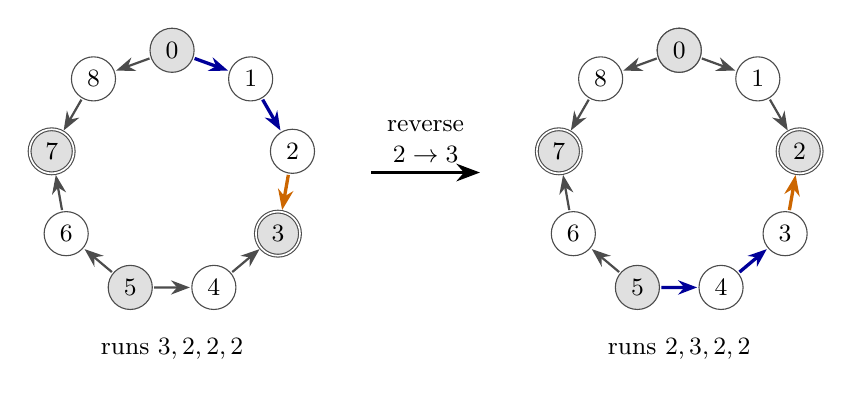
\begin{tikzpicture}[scale=1.15]
\foreach \side/\dx in {L/0,R/5.6}{
  \foreach \v in {0,...,8}{ \coordinate (\side\v) at ($(\dx,0)+(90-40*\v:1.35)$); }
}
\node[src] (a0) at (L0) {0}; \node[vtx] (a1) at (L1) {1}; \node[vtx] (a2) at (L2) {2};
\node[snk] (a3) at (L3) {3}; \node[vtx] (a4) at (L4) {4}; \node[src] (a5) at (L5) {5};
\node[vtx] (a6) at (L6) {6}; \node[snk] (a7) at (L7) {7}; \node[vtx] (a8) at (L8) {8};
\draw[longp] (a0)--(a1); \draw[longp] (a1)--(a2); \draw[hot] (a2)--(a3);
\draw[arc] (a5)--(a4); \draw[arc] (a4)--(a3);
\draw[arc] (a5)--(a6); \draw[arc] (a6)--(a7);
\draw[arc] (a0)--(a8); \draw[arc] (a8)--(a7);
\node[font=\small] at (0,-1.95) {runs $3,2,2,2$};
\node[vtx] (b0) at (R0) {0}; \node[vtx] (b1) at (R1) {1}; \node[snk] (b2) at (R2) {2};
\node[vtx] (b3) at (R3) {3}; \node[vtx] (b4) at (R4) {4}; \node[src] (b5) at (R5) {5};
\node[vtx] (b6) at (R6) {6}; \node[snk] (b7) at (R7) {7}; \node[vtx] (b8) at (R8) {8};
\node[src] at (R0) {0};
\draw[arc] (b0)--(b1); \draw[arc] (b1)--(b2); \draw[hot] (b3)--(b2);
\draw[longp] (b5)--(b4); \draw[longp] (b4)--(b3);
\draw[arc] (b5)--(b6); \draw[arc] (b6)--(b7);
\draw[arc] (b0)--(b8); \draw[arc] (b8)--(b7);
\node[font=\small] at (5.6,-1.95) {runs $2,3,2,2$};
\draw[-{Stealth[length=3mm]},thick] (2.2,0) -- node[above,font=\small,align=center]{reverse\\ $2\to3$} (3.4,0);
\end{tikzpicture}
\caption{\Cref{thm:cycles} for $C_9$ and $w=2$ ($n=2\cdot2\cdot2+1$). The orientation has runs of lengths $3,2,2,2$ and height $3$. The only binding moves pass the excess unit of the long run (blue) to a neighbouring run; here reversing $2\to3$ makes the run $5\to4\to3\to2$ the long one. The $18$ orientations of this kind and their $131{,}040$ states form a recurrent class, and the cycle $C_9$ has odd girth $9>2w+1$.}
\label{fig:c9}
\end{figure}

\begin{table}[t]
\centering\small
\caption{Recurrent classes of excessive height on cycles (\cref{thm:cycles}). Rows list every pair with $n\le13$ and $n\equiv1\pmod{2w}$; for all other pairs with $3\le n\le14$ and $1\le w\le n-2$ there is none. All entries are certified (\texttt{cycle\_classification.json}). The pairs with $w=1$ have $\chi(C_n)=3>w+1$ and lie outside the conjecture's hypothesis.}
\label{tab:cycles}
\begin{tabular}{rrlrr}
\toprule
$n$ & $w$ & run lengths & linear extensions $e_{n,w}$ & states $2n(n+1)e_{n,w}$\\
\midrule
5 & 2 & 3,2 & 3 & 180\\
7 & 3 & 4,3 & 10 & 1{,}120\\
9 & 2 & 3,2,2,2 & 728 & 131{,}040\\
9 & 4 & 5,4 & 35 & 6{,}300\\
11 & 5 & 6,5 & 126 & 33{,}264\\
13 & 2 & 3,2,2,2,2,2 & 1{,}010{,}328 & 367{,}759{,}392\\
13 & 3 & 4,3,3,3 & 101{,}420 & 36{,}916{,}880\\
13 & 6 & 7,6 & 462 & 168{,}168\\
\midrule
$2r+1$ & 1 & 2,1,\dots,1 & & e.g.\ 480 for $n=5$\\
\bottomrule
\end{tabular}
\end{table}

\what{For $w\ge2$, every cycle satisfies the colouring hypothesis, and under (PR) the conjecture holds on $C_n$ exactly when $n\not\equiv1\pmod{2w}$; otherwise it fails in exactly one recurrent class of excessive height. (At $w=1$, odd cycles lie outside the hypothesis.) Long odd cycles do not help: $C_9$ at $w=2$ fails although its odd girth is $9>2w+1$. Even cycles satisfy the conjecture under (PR), at every cap. Any repair of the conjecture must therefore involve arithmetic between cycle lengths and $w$, not just lengths of odd cycles.}

\section{Beyond cycles}\label{sec:beyond}

\subsection{Two odd cycles joined by a path}\label{sec:twocycles}

Let $a,b\ge1$ and $L\ge0$. The graph $G(a,b,L)$ consists of an odd cycle $C_{2a+1}$ through a vertex $\alpha$, an odd cycle $C_{2b+1}$ through a vertex $\beta$, and a path with $L$ edges from $\beta$ to $\alpha$; for $L=0$, $\alpha=\beta$. It has $n=2a+2b+L+1$ vertices and $\chi=3$. Let $\K$ be the set of four orientations in which $C_{2b+1}$ is balanced with sink $\beta$, the path is directed from $\beta$ to $\alpha$, and $C_{2a+1}$ is balanced with source $\alpha$. There are two choices of the source of $C_{2b+1}$ and two of the sink of $C_{2a+1}$; see \cref{fig:twocycles}.

\begin{theorem}[Two odd cycles]\label{thm:twocycles}
Let $w=a+b+L+1$. On $G(a,b,L)$ with cap $w$, the states with orientation in $\K$ form a set that is closed for every admissible rate function. Under (PR) it is a recurrent class of height $w+1$ with $4(n+1)\binom{2a-1}{a-1}\binom{2b-1}{b-1}$ states. Since $\chi=3\le w+1$, this contradicts Conjecture~1. The four reversed orientations, in which $C_{2a+1}$ has sink $\alpha$, the path is directed from $\alpha$ to $\beta$, and $C_{2b+1}$ has source $\beta$, likewise form a closed set and, under (PR), a second recurrent class of excessive height, disjoint from the first. When $L=0$ the junction vertex $\alpha=\beta$ is the sink of one balanced cycle and the source of the other, and the condition on the path is empty.
\end{theorem}

\begin{proof}
\emph{Goal: compute depths and list the moves.} On $C_{2b+1}$, write the balanced orientation with source $s'$, long path $s'\to s'_1\to\dots\to\beta$ ($b+1$ edges) and a short path with $b$ edges. On $C_{2a+1}$, write it with source $\alpha$, long path $\alpha\to\dots\to t'_1\to t'$ ($a+1$ edges) and a short path with $a$ edges. Depths increase along the chain: $\dep(\beta)=b+1$, $\dep(\alpha)=b+1+L$, and on $C_{2a+1}$ the depth equals $b+1+L$ plus the distance from $\alpha$ along its run. So $\dep(t')=w+1$ and $\dep(t'_1)=w$. The predecessor of $t'$ on the short path has depth $w-1$, and every other vertex has depth at most $w-1$. By \cref{lem:moves}(a) the only upper move reverses $t'_1\to t'$, which moves the sink of $C_{2a+1}$ and keeps it balanced with source $\alpha$. Dually, $\up(s')=w+1$, $\up(s'_1)=w$, and every other vertex with an in-neighbour has $\up\le w-1$. The only lower move reverses $s'\to s'_1$, which moves the source of $C_{2b+1}$ and keeps it balanced with sink $\beta$.

\emph{Goal: closure and connectivity.} Both moves stay in $\K$, and the closure uses only \cref{lem:moves}(a). They act independently on the two cycles and are involutions, so the four orientations form a square in $\G_w$. Under (PR) both occur (\cref{lem:moves}(b)), and \cref{cor:reduction} gives a recurrent class.

\emph{Goal: count.} $P_A$ is the ordinal sum of the poset on $C_{2b+1}$, the path and the poset on $C_{2a+1}$. Its linear extensions are counted as in \cref{thm:balanced}. The reversed family follows by exchanging the queues.
\end{proof}

\begin{figure}[t]
\centering
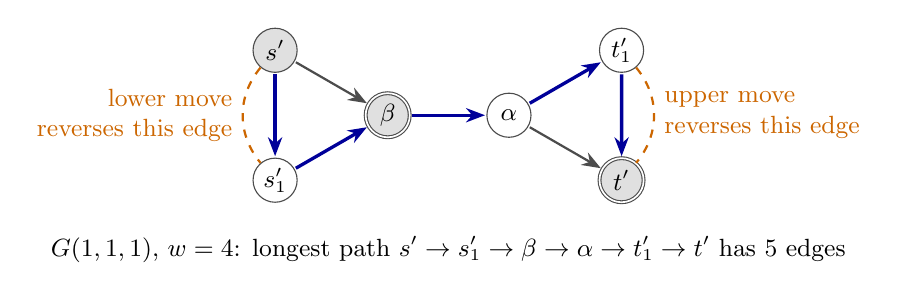
\begin{tikzpicture}[scale=1.1]
\node[src] (b2) at (0,0.75) {$s'$};
\node[vtx] (b1) at (0,-0.75) {$s'_1$};
\node[snk] (b0) at (1.3,0) {$\beta$};
\node[vtx] (a0) at (2.7,0) {$\alpha$};
\node[vtx] (a1) at (4.0,0.75) {$t'_1$};
\node[snk] (a2) at (4.0,-0.75) {$t'$};
\draw[longp] (b2)--(b1); \draw[longp] (b1)--(b0); \draw[arc] (b2)--(b0);
\draw[longp] (b0)--(a0);
\draw[longp] (a0)--(a1); \draw[longp] (a1)--(a2); \draw[arc] (a0)--(a2);
\node[font=\small,align=center] at (2.0,-1.55) {$G(1,1,1)$, $w=4$: longest path $s'\to s'_1\to\beta\to\alpha\to t'_1\to t'$ has $5$ edges};
\draw[orange!80!black,dashed,thick] (b2) to[bend right=40] node[left,font=\small,align=right]{lower move\\reverses this edge} (b1);
\draw[orange!80!black,dashed,thick] (a1) to[bend left=40] node[right,font=\small,align=left]{upper move\\reverses this edge} (a2);
\end{tikzpicture}
\caption{\Cref{thm:twocycles} for two triangles joined by an edge, $w=a+b+L+1=4$. The two binding moves (dashed) reverse $s'\to s'_1$ and $t'_1\to t'$. They move the source of the left triangle and the sink of the right triangle, and the longest path keeps $w+1=5$ edges.}
\label{fig:twocycles}
\end{figure}

For two triangles sharing a vertex ($a=b=1$, $L=0$) the theorem gives a counterexample at $w=3$ on five vertices with $24$ states. For two triangles joined by an edge it gives $w=4$. The census below shows that the same graph also fails at $w=2$, with a different class of eight orientations. We also computed every recurrent class of excessive height on $G(a,b,L)$ for $1\le a\le b\le3$, $0\le L\le3$ and $n\le10$, at every cap $w\ge2$ (\texttt{two\_cycle\_family.json}). Apart from the two families of \cref{thm:twocycles}, every such class has $4r$ orientations and occurs at a cap $w$ with $a+b+L+1=rw$ for some $r\ge2$. Such classes occur for six of the ten pairs $(G(a,b,L),w)$ of this kind in the range; there is none, for example, for $G(1,2,0)$ or $G(2,2,1)$ at $w=2$. These classes resemble the patterns $\Pat_{n,w}$ with $r\ge2$ in \cref{thm:cycles}, but we do not prove a general statement about them.

\subsection{All small graphs}\label{sec:census}

By \cref{cor:reduction}, under (PR) the conjecture for $(G,w)$ is a finite question about $\G_w$. We answered it exactly for every connected graph with $3\le n\le7$ vertices and every cap $w$ with $\chi(G)\le w+1\le n-1$; caps $w\ge n-1$ admit no high orientation. The graphs were generated by our own program and counted against the On-Line Encyclopedia of Integer Sequences~\cite{OEIS} (A000088 and A001349). The binding moves were obtained by simulating every transition from every state, not from \cref{lem:moves}. \Cref{tab:census} summarises the result.

\begin{table}[t]
\centering\small
\caption{Census of connected graphs on $n$ vertices (exact; \texttt{census\_small\_graphs.json}). ``Eligible'' counts graphs with $\chi(G)\le w+1$; ``violating'' counts those with a recurrent class of height $>w$ under (PR). Pairs with $n\le4$ have no violations. In total there are $79$ violating pairs with $n\le6$ and $1355$ with $n\le7$. None is bipartite, and none has $w=1$.}
\label{tab:census}
\begin{tabular}{rrrrr}
\toprule
$n$ & $w$ & eligible graphs & violating graphs & bipartite (all non-violating)\\
\midrule
5 & 1 & 5 & 0 & 5\\
5 & 2 & 17 & 1 & 5\\
5 & 3 & 20 & 5 & 5\\
6 & 1 & 17 & 0 & 17\\
6 & 2 & 81 & 3 & 17\\
6 & 3 & 107 & 46 & 17\\
6 & 4 & 111 & 24 & 17\\
7 & 1 & 44 & 0 & 44\\
7 & 2 & 519 & 26 & 44\\
7 & 3 & 801 & 518 & 44\\
7 & 4 & 847 & 442 & 44\\
7 & 5 & 852 & 290 & 44\\
\bottomrule
\end{tabular}
\end{table}

Three features stand out. First, for $w\ge3$ violations are common: on seven vertices, $518$ of the $801$ eligible graphs violate the conjecture at $w=3$, and $442$ of $847$ at $w=4$. Second, at $w=2$ the only violating graph on five vertices is $C_5$. Every other violating graph on at most seven vertices contains two triangles, and all of its recurrent classes of excessive height have exactly eight orientations. Third, no bipartite graph in the census violates the conjecture at any cap; \cref{sec:bipartite} proves this for all bipartite graphs at odd caps under (PR). Every recurrent class of excessive height in the census has height $w+1$ or $w+2$.

\subsection{Several jobs per class}\label{sec:multiplicity}

Suppose class $v$ has $m_v\ge1$ jobs. Jobs of one class never swap, since the swapping graph has no loops. Dorsman and Gardner's relabelling~\cite[Remark~9]{DG2024} gives each job its own class. The resulting \emph{blow-up} $G^{(m)}$ replaces $v$ by $m_v$ pairwise non-adjacent twins with the neighbours of $v$, and the rate functions treat twins as the original class. Then $\chi(G^{(m)})=\chi(G)$, and the source states the conjecture for several jobs per class through this relabelling.

\begin{proposition}[Reduction to one job per class]\label{prop:multiplicity}
Assume the canonical symmetric lift of both queues' rate functions: in the blow-up system, every twin of $v$ has exactly the rates of class $v$, in each queue, so that the rate functions are invariant under permutations of twins. Then a state of the system with multiplicities $m$ is recurrent if and only if one (equivalently, every) relabelled state of the blow-up system is recurrent.
\end{proposition}

\begin{proof}
Forgetting the labels maps the blow-up chain onto the original chain, and every transition of the original chain lifts from every preimage. Hence the original chain is a lumping of the blow-up chain. Moreover, by the symmetric lift, permuting twins maps transitions to transitions with the same rates, so it is an automorphism of the blow-up chain. Suppose a lift $x$ is recurrent and $\bar y$ is reachable from its image $\bar x$. Lifting the path gives some $y$ over $\bar y$, reachable from $x$; then $x$ is reachable from $y$, and projecting shows that $\bar x$ is reachable from $\bar y$. Conversely, suppose $\bar x$ is recurrent and $y$ is reachable from a lift $x$. Then $\bar x$ is reachable from $\bar y$, so $y$ reaches some lift $\sigma x$, with $\sigma$ a permutation of twins. Applying $\sigma$ repeatedly to the path from $x$ to $\sigma x$ leads from $\sigma x$ to $\sigma^2x,\dots,\sigma^jx=x$, where $j$ is the order of $\sigma$. So $y$ reaches $x$, and $x$ is recurrent.
\end{proof}

\begin{table}[t]
\centering\small
\caption{Several jobs per class (exact; \texttt{multiplicity\_check.json}). ``High class'' means a recurrent class of height $>w$ under (PR).}
\label{tab:mult}
\begin{tabular}{l>{\raggedright\arraybackslash}p{6.2cm}ll}
\toprule
graph & multiplicities & caps & high class?\\
\midrule
$C_5$ & $(1,1,1,1,1)$ & $w=2$ & yes (180 states)\\
$C_5$ & all vectors in $\{1,2,3\}^5$ with $6$ to $8$ jobs, up to rotation and reflection ($8$ vectors) & $w=2$ & no\\
$C_7$ & one or two classes doubled & $w=3$ & no\\
$C_9$ & one class doubled & $w=2$, $w=4$ & no\\
$K_3$ & $(2,2,1)$ & $w=3$ & yes\\
$K_3$ & $(2,2,2)$ & $w=3$, $w=4$ & yes\\
bowtie & one class doubled & $w=3$ & yes\\
\bottomrule
\end{tabular}
\end{table}

\Cref{tab:mult} shows what happens. On the cycles we examined, a single extra job destroys every recurrent class of excessive height. In general, however, extra jobs do not restore the conjecture. The triangle with two jobs in every class ($6$ jobs, $\chi=3\le w+1$) has recurrent classes of excessive height at $w=3$ and $w=4$.

\what{The failure of the conjecture is not a quirk of odd cycles or of one job per class. Under (PR), the census, \cref{thm:twocycles} and \cref{tab:mult} show that among small graphs it is common once $w\ge3$ and the graph has a few odd cycles. What the data single out is bipartiteness: no bipartite example we computed violates the conjecture.}

\section{Where the conjecture holds: bipartite graphs}\label{sec:bipartite}

\begin{theorem}[Bipartite graphs, odd caps]\label{thm:bipartite}
Let $G$ be bipartite, let $w\ge1$ be odd, and assume (PR). Then every state of height greater than $w$ is transient. In particular Conjecture~1 holds for every bipartite swapping graph at $w=1$ under (PR).
\end{theorem}

\begin{proof}
\emph{Goal: a quantity that every suitable move increases.} Let $X\cup Y$ be a bipartition of $G$, and call an edge \emph{good} if it is oriented from $X$ to $Y$. The orientation in which all edges are good has height $1\le w$. Recall the two moves of \cref{lem:moves} with $D=V$ or its dual. \emph{Sinking} a vertex $v$ with $\dep(v)\ge w$ reverses all its out-edges. \emph{Raising} a vertex $v$ with $\up(v)\ge w$ reverses all its in-edges. Sinking $v\in Y$ makes every edge at $v$ good and changes no other edge. If $v$ had an out-edge, this strictly increases the number of good edges. Similarly, raising $v\in X$ with an in-edge strictly increases it.

\emph{Goal: such a move exists whenever the height exceeds $w$.} Let $z_0\to z_1\to\cdots\to z_h$ be a longest directed path, with $h\ge w+1$. Then $\dep(z_j)=j$ and $\up(z_j)=h-j$. For $w\le j\le h-1$, the vertex $z_j$ has depth at least $w$ and the out-neighbour $z_{j+1}$, so it can be sunk; this improves if $z_j\in Y$. For $1\le j\le h-w$, the vertex $z_j$ has $\up\ge w$ and the in-neighbour $z_{j-1}$, so it can be raised; this improves if $z_j\in X$. Suppose no improving move exists. Then $z_j\in X$ for every $j\in[w,h-1]$. Consecutive vertices of the path lie in different parts, so this interval has a single element and $h=w+1$, with $z_w\in X$. Likewise $z_j\in Y$ for $j\in[1,h-w]=\{1\}$. But $z_1$ and $z_w$ are $w-1$ steps apart, an even number since $w$ is odd, so they lie in the same part. This is a contradiction.

\emph{Conclusion.} Each improving move strictly increases the number of good edges, which is at most $|E|$. So a finite sequence of moves reaches an orientation of height at most $w$, from which (\cref{cor:reduction}(ii)) there is no return.
\end{proof}

For even $w$ the argument stops at configurations where every longest path has exactly $w+1$ edges and runs from $X$ to $Y$. We could not exclude such traps in general. The computations, however, find none.

\begin{conjecture}[Bipartite swapping graphs]\label{conj:bipartite}
For every bipartite swapping graph, every cap $w\ge1$ and positive rates, every state of height greater than $w$ is transient.
\end{conjecture}

The conjecture is certified for every connected bipartite graph with at most nine vertices and every cap $1\le w\le n-2$. These are the $182$ graphs on eight and the $730$ on nine vertices, counted against A033995 and A005142~\cite{OEIS} (\texttt{bipartite\_check.json}, \texttt{bipartite\_check\_n9.json}). It is also certified for every connected bipartite graph with at most seven vertices and every cap when \emph{only the heads of the queues are served}. That is the weakest positivity allowed by the order-independent conditions, and the one in which Dorsman and Gardner expected the real difficulty~\cite[Appendix~C.2]{DG2024}. Even cycles satisfy the conjecture at every cap by \cref{thm:cycles}.

\what{Under (PR), the original conjecture is true in the setting of all of its source's examples: bipartite graphs at $w=1$. More generally it is true for bipartite graphs at every odd cap. Every counterexample we know contains an odd cycle, and the proof above shows how parity along a longest path enters. A plausible corrected statement replaces ``$(w+1)$-partite'' by ``bipartite''.}

\section{Stationary laws on the balanced class}\label{sec:stationary}

The conjecture was meant to guarantee product form. We now ask what the stationary law looks like on the class of \cref{thm:balanced}, where the conjecture fails. Throughout, $w\ge2$, $n=2w+1$, (PR) holds and rates are additive.

For a balanced orientation with source $s$ and sink $t$, every full-queue word has the form $s\,\omega\,t$, where $\omega$ interleaves the long-path vertices $x_1,\dots,x_w$ with the short-path vertices $y_1,\dots,y_{w-1}$. We record $\omega$ as a word $\theta\in\{\mathrm X,\mathrm Y\}^{2w-1}$ with $w$ letters $\mathrm X$; the $i$-th $\mathrm X$ stands for $x_i$ and the $i$-th $\mathrm Y$ for $y_i$. Let $M_w=2n\binom{2w-1}{w-1}=n!/(w!)^2$ be the number of balanced global words.

\begin{lemma}[Head map]\label{lem:head}
The capped service of the head of a full upper queue maps the $M_w$ full-upper states of $\Bal_w$ bijectively onto the $M_w$ states of $\Bal_w$ with one job in the lower queue. If $\theta=\mathrm Y\theta_0$, the transition does not bind; the orientation is unchanged and the new letter word is $\theta_0\mathrm Y$. If $\theta=\mathrm X\theta_0$, it binds; the new orientation has the same source and the other sink, and in its own long/short convention the new letter word is $\overline{\theta_0}\,\mathrm X$, where the bar exchanges $\mathrm X$ and $\mathrm Y$. Encoding a state by a bit for the sink choice followed by its letters (with $\mathrm X=1$, complemented for the second sink choice), the map is cyclic rotation of binary words of length $2w$ with $w$ ones. The same holds for the lower queue.
\end{lemma}

\begin{proof}
If $\theta_1=\mathrm Y$, the scan follows $s\to y_1\to\dots\to y_{w-1}\to t$ and ends at $t$, the last job, after $w$ replacements without binding. If $\theta_1=\mathrm X$, it follows $s\to x_1\to\dots\to x_w$ and the cap ejects $x_w$, which has the later neighbour $t$. Then $s$ occupies the slot of $x_1$, each $x_i$ that of $x_{i+1}$, and $x_w$ joins the lower queue. By \cref{thm:balanced} the new orientation has sink $x_w$; its long path is $s,y_1,\dots,y_{w-1},t,x_w$. Reading off the letters gives $\overline{\theta_0}\,\mathrm X$, the final $\mathrm X$ being $t$. The rotation property follows by checking the four cases of first bit and first letter. A rotation is a bijection.
\end{proof}

By \cref{prop:promotion}, the \emph{uncapped} head map on a full queue is promotion. Promotion is a bijection of each set of linear extensions, and in the letter description it moves the first letter to the end.

\subsection{Homogeneous rates}

\begin{theorem}[Homogeneous law]\label{thm:homog}
Let every job be served at rate $\mu_0>0$ in the upper queue and $\nu_0>0$ in the lower queue. The unique stationary distribution on $\Bal_w$ is
\[
 \pi(c;d)=\frac1{M_w}\binom{n}{k}p^k(1-p)^{n-k},\qquad k=|c|,\quad p=\frac{\nu_0}{\mu_0+\nu_0}.
\]
So the global word is uniform on its $M_w$ values and independent of the split $k$, which is binomial. Equivalently, $\pi$ is proportional to the product weight $q(c;d)=\mu_0^{-k}\nu_0^{-(n-k)}/(k!\,(n-k)!)$.
\end{theorem}

\begin{proof}
\emph{Goal 1: the uncapped weights.} Here $\Delta\mu\equiv\mu_0$, so $\mu(c_1,\dots,c_j)=j\mu_0$ and the product-form factor of the upper queue is $\Phi_\mu(c)=\mu_0^{-k}/k!$; similarly for the lower queue. Hence $q=\Phi_\mu\Phi_\nu$ is the product form of~\cite[Theorem~5]{CD2021} (\cite[Theorem~3]{DG2024}). On each $\Sg_A$, which is irreducible by \cref{lem:fixed}, $q$ is stationary for the uncapped chain.

\emph{Goal 2: compare the two generators.} Both chains have the same total outflow rate $k\mu_0+(n-k)\nu_0$ at every state. They differ only at binding transitions, which by \cref{rem:heads} are head services from full queues. Fix a target state $\tau$ with one lower job. By \cref{lem:head} it has exactly one capped head-predecessor. By bijectivity of promotion, together with \cref{lem:nonbinding}, it also has exactly one uncapped head-predecessor. Both predecessors are full-upper states, with the same weight $\mu_0^{-n}/n!$ and the same rate $\mu_0$. So the inflows into $\tau$ agree. States with one upper job are treated in the same way, and all other inflows are identical. Hence $q$ satisfies the global balance of the capped chain. Summing $q$ over the $M_w$ words and $n+1$ splits gives the normalisation, and irreducibility gives uniqueness.
\end{proof}

\begin{proposition}[Partial balance]\label{prop:partial}
The law of \cref{thm:homog} satisfies the partial-balance equations (23)--(24) of~\cite{DG2024}: at every state of $\Bal_w$, the outflow due to upper (respectively lower) services equals the inflow due to lower (respectively upper) services.
\end{proposition}

\begin{proof}
The uncapped product form satisfies these equations on each $\Sg_A$ (the proof of~\cite[Theorem~5]{CD2021}; \cite[Appendix~B]{DG2024}). The capped equations differ only through the binding head events. Each such event is a lower-queue service entering a state with one upper job, or an upper-queue service entering a state with one lower job. In each of these equations the capped and uncapped inflows come from one full-queue predecessor each, with equal weight and rate, as in the proof of \cref{thm:homog}.
\end{proof}

\what{Under homogeneous rates the failure of the conjecture does not destroy product form. The recurrent class of excessive height carries exactly the original product weights, even in Dorsman and Gardner's stronger partial-balance sense. A computation that keeps only the low orientations would miss this class entirely, although its law is as simple as theirs.}

\subsection{Heterogeneous rates}

A natural repair is to keep the original factors and allow one free positive constant per orientation. We show that, on the high class $\Bal_w$ of $C_{2w+1}$ and for additive per-job rates, this works only in the homogeneous case, for every $w\ge2$. (On a low orientation the cap never binds, and the ordinary product form holds for any rates~\cite[Theorem~7]{DG2024}.)

\begin{theorem}[Orientation-scaled product form]\label{thm:hetero}
Let $w\ge2$ and $G=C_{2w+1}$, and let the rates be additive: job $i$ is served at rate $\mu_i>0$ in the upper queue and $\nu_i>0$ in the lower queue. There exist positive constants $(\kappa_A)_{A\in\Obal_w}$ such that
\[
 \pi(c;d)\ \propto\ \kappa_{\Or(c;d)}\,\Phi_\mu(c)\,\Phi_\nu(d)
\]
is stationary on the balanced class $\Bal_w$ if and only if $\mu_0=\dots=\mu_{n-1}$ and $\nu_0=\dots=\nu_{n-1}$. (The two constants may differ.)
\end{theorem}

\begin{proof}
``If'' is \cref{thm:homog}, with $\kappa$ constant. For ``only if'' we proceed in four steps.

\emph{Step 1: where balance can fail.} With $q=\Phi_\mu\Phi_\nu$, the uncapped chain has $q$ stationary on each $\Sg_A$, as in the proof of \cref{thm:homog}. The capped and uncapped chains have the same outflows. They differ only at head services of full queues (\cref{rem:heads}). The global-balance residual of $\kappa q$ therefore vanishes except at targets $\tau$ of binding head services. Consider such a $\tau$ with one lower job. Let $F$ be its capped predecessor, a full-upper state in an orientation $A'$, and $F'$ its uncapped predecessor, a full-upper state in $A=\Or(\tau)$. Balance at $\tau$ reads $\kappa_{A'}\,\mu_s\,\Phi_\mu(F)=\kappa_A\,\mu_s\,\Phi_\mu(F')$, where $s$ is the common source and head. That is,
\[
\frac{\kappa_{A'}}{\kappa_A}=\frac{\Phi_\mu(F')}{\Phi_\mu(F)}.
\]

\emph{Step 2: the two predecessors explicitly.} Let $A'$ have source $s$, long path $s,x_1,\dots,x_w,t$ and short path $s,y_1,\dots,y_{w-1},t$, and let $F$ have letter word $\mathrm X\theta_0$, where $\theta_0$ has $w-1$ letters of each kind. By \cref{lem:head}, $\tau$ has the word $s\,\omega'\,t\,x_w$, where $\omega'$ follows the pattern $\theta_0$ with $\mathrm X\mapsto x_1,\dots,x_{w-1}$ and $\mathrm Y\mapsto y_1,\dots,y_{w-1}$. One checks directly that its uncapped head-predecessor in $A$ is
\[
F' = s\,y_1\,\omega''\,x_w,\qquad\text{where }\omega''\text{ follows }\theta_0\text{ with }\mathrm X\mapsto x_1,\dots,x_{w-1},\ \mathrm Y\mapsto y_2,\dots,y_{w-1},t;
\]
the uncapped scan from $s$ runs $s\to y_1\to\dots\to y_{w-1}\to t\to x_w$. Meanwhile $F=s\,x_1\,\omega\,t$, where $\omega$ follows $\theta_0$ with $\mathrm X\mapsto x_2,\dots,x_w$ and $\mathrm Y\mapsto y_1,\dots,y_{w-1}$.

\emph{Step 3: a lattice-path formula.} After the first $2+j$ letters, where $\theta_0$ has contributed $\xi$ letters $\mathrm X$ and $\eta$ letters $\mathrm Y$ ($\xi+\eta=j$), the prefix of $F$ is $\{s,x_1,\dots,x_{\xi+1},y_1,\dots,y_\eta\}$. The prefix of $F'$ is $\{s,x_1,\dots,x_\xi,y_1,\dots,y_{\eta+1}\}$, with $y_w:=t$. Let $\rho(\xi,\eta)=\mu_s+\sum_{i\le \xi}\mu_{x_i}+\sum_{i\le \eta}\mu_{y_i}$. The prefixes of length $1$ and $n$ coincide. Hence
\[
\frac{\Phi_\mu(F')}{\Phi_\mu(F)}=\prod_{(\xi,\eta)}f(\xi,\eta),\qquad f(\xi,\eta)=\frac{\rho(\xi,\eta)+\mu_{x_{\xi+1}}}{\rho(\xi,\eta)+\mu_{y_{\eta+1}}},
\]
where $(\xi,\eta)$ runs over the $2w-1$ lattice points visited by the monotone path from $(0,0)$ to $(w-1,w-1)$ that $\theta_0$ describes ($\mathrm X$ is a step in $\xi$, $\mathrm Y$ a step in $\eta$). By Step~1 this product must not depend on $\theta_0$. Two paths that go around one unit square in the two possible ways, and agree elsewhere, force $f(\xi+1,\eta)=f(\xi,\eta+1)$.

\emph{Step 4: the corner identities force constant rates.} Number the vertices so that $x_i=s+\delta i$ and $y_i=s-\delta i$, where $\delta=\pm1$; this includes $y_w=t$. The square at $(0,0)$ gives $f(1,0)=f(0,1)$, that is,
\[
(\mu_s+\mu_{s+\delta}+\mu_{s+2\delta})(\mu_s+\mu_{s-\delta}+\mu_{s-2\delta})=(\mu_s+\mu_{s+\delta}+\mu_{s-\delta})^2,
\]
that is, $\Omega_{s+\delta}\Omega_{s-\delta}=\Omega_s^2$, where $\Omega_v=\mu_{v-1}+\mu_v+\mu_{v+1}$. Every source $s$ occurs, so $\Omega_{v+1}/\Omega_v$ is constant around the cycle. Its $n$-th power is $1$ and it is positive, so it equals $1$ and $\Omega$ is constant. Then $\mu_{v+2}=\Omega_{v+1}-\Omega_v+\mu_{v-1}=\mu_{v-1}$, so $\mu$ has period $3$ as well as period $n$. If $3\nmid n$, $\mu$ is constant. If $3\mid n$, then $n\ge9$ and $w\ge4$, and the square at $(1,0)$, which gives $f(2,0)=f(1,1)$, is available. Write $(\mu_s,\mu_{s+1},\mu_{s+2})=(\lambda_0,\lambda_1,\lambda_2)$ and $T=\lambda_0+\lambda_1+\lambda_2$; by periodicity $\mu_{s+3}=\lambda_0$, $\mu_{s-1}=\lambda_2$ and $\mu_{s-2}=\lambda_1$. With $\delta=1$ this square gives $(T+\lambda_0)(T+\lambda_1)=(T+\lambda_2)^2$, and replacing $s$ by $s+1$ and $s+2$ gives $(T+\lambda_1)(T+\lambda_2)=(T+\lambda_0)^2$ and $(T+\lambda_2)(T+\lambda_0)=(T+\lambda_1)^2$. Dividing the first identity by the second gives $(T+\lambda_0)^3=(T+\lambda_2)^3$, so $\lambda_0=\lambda_2$, and then the first identity gives $\lambda_1=\lambda_0$. So $\mu$ is constant. Exchanging the queues reverses orientations, exchanges $\mu$ and $\nu$, and maps $\Bal_w$ to itself. The same argument therefore shows that $\nu$ is constant.
\end{proof}

\begin{corollary}\label{cor:onerate}
With rates $(1,\dots,1,a)$ in both queues, the orientation-scaled product form is stationary on $\Bal_w$ if and only if $a=1$, for every $w\ge2$. Concretely, the corner identity at the source two steps before the changed job reads $3(2+a)=9$.
\end{corollary}

\begin{example}[Two explicit equations on $C_5$]\label{ex:c5rows}
For $w=2$ and rates $(1,1,1,1,a)$ in both queues, label the orientations by bits $b_0\cdots b_4$, with $b_i=1$ if $i$ precedes $i+1$ in the global word. Let $O_1=00011$ and $O_2=00111$, and $Q_a=(a+1)(a+2)(a+3)(a+4)$. Consider the states $u=((2);(0,1,4,3))$ and $v=((2);(0,4,1,3))$, both in $O_2$. Their global-balance equations under the ansatz reduce to
\[
\frac{\kappa_{O_1}}{6(a+3)(a+4)}=\frac{\kappa_{O_2}}{Q_a},\qquad \frac{\kappa_{O_1}}{2(a+2)(a+3)(a+4)}=\frac{\kappa_{O_2}}{Q_a}.
\]
They give $\kappa_{O_2}/\kappa_{O_1}=(a+1)(a+2)/6$ and $\kappa_{O_2}/\kappa_{O_1}=(a+1)/2$, which differ by $(a+1)(a-1)/6$. These are exact identities in the indeterminate $a$, and the package lists every predecessor event (\texttt{symbolic\_rate\_certificate.json}).
\end{example}

\paragraph{How large is the deviation, and which class is reached?} \Cref{thm:hetero} rules out one representation. The true stationary law on $\Bal_2$ exists and is computed exactly in \cref{tab:deviation}. Rescaling the original factors so that every orientation receives its true mass leaves an error below $2\times10^{-3}$ in total variation, for the rates we computed. With a single normalising constant the error is larger. Both laws give mean upper-queue length $n/2$, but this is forced by queue-exchange symmetry (the same rates are used in both queues) and is not evidence of accuracy.

The chain is not ergodic. On $C_5$ with $w=2$ there are eleven recurrent classes, so the long-run behaviour depends on the initial state. With unit rates, the $60$ transient states are absorbed into $\Bal_2$ with probability $1/7$ (forty states) or $2/7$ (twenty states). From a uniformly random initial state, the long-run probability of being in $\Bal_2$ is exactly $67/252\approx0.266$.

\begin{table}[t]
\centering\small
\caption{Exact stationary law on $\Bal_2$ for rates $(1,1,1,1,a)$ in both queues, compared with the original weights $q$ (\texttt{stationary\_details.json}). ``Orientation-matched'' rescales $q$ within each orientation to the true orientation mass. ``Spread'' is the largest value, over orientations, of $\max(\pi/q)/\min(\pi/q)$ within that orientation.}
\label{tab:deviation}
\begin{tabular}{rrrr}
\toprule
$a$ & TV to normalised $q$ & TV to orientation-matched $q$ & spread of $\pi/q$\\
\midrule
$1/2$ & $0.0494$ & $4.1\times10^{-4}$ & $1.012$\\
$2$ & $0.1114$ & $7.9\times10^{-4}$ & $1.019$\\
$10$ & $0.3496$ & $1.8\times10^{-3}$ & $1.149$\\
\bottomrule
\end{tabular}
\end{table}

\what{With different job rates, the product weights do not survive on the class of excessive height, even after reweighting each orientation; the failure is exact but small. For performance estimates, the practical lesson is that the closed tandem with bounded swaps can be non-ergodic. Which recurrent class the system settles in, and hence its long-run law, depends on how it is started.}

\section{Discussion}\label{sec:discussion}

\paragraph{What survives of the conjecture.} The motivating corollary, read classwise (every recurrent class lies in a single low orientation and carries its product-form law), fails for two reasons. First, recurrent classes of excessive height exist (\cref{thm:balanced,thm:cycles,thm:twocycles}). Second, on $\Bal_w$ their laws are not orientation-scaled product forms once the additive rates vary within a queue (\cref{thm:hetero}). Several statements remain true:
\begin{itemize}
\item every low orientation forms a closed class with the product-form law~\cite[Theorem~7]{DG2024}. So under the colouring condition \emph{some} recurrent class has height at most $w$. This is already in the source and cannot be strengthened to \emph{every} recurrent class;
\item the conjecture holds, under (PR), for bipartite graphs at odd caps (\cref{thm:bipartite}), for even cycles at all caps, and for $w\ge2$ on $C_n$ with $n\not\equiv1\pmod{2w}$ (\cref{thm:cycles});
\item one proposed repair, assuming odd girth larger than $2w+1$, is false (\cref{thm:cycles}: $C_{4w+1}$).
\end{itemize}

\paragraph{The swap-limit programme.} For the redundancy question that motivated caps, our results concern fixed caps only. They show that the invariant-set argument of~\cite{DG2024} cannot cover every $(w+1)$-colourable swapping graph, because on some of them (for example $C_{2w+1}$) the process can remain forever in orientations where the cap binds. They also show that the product form can nevertheless survive there (\cref{thm:homog}). Any proof for random state-dependent caps will need to account for such classes.

\paragraph{Open problems.}
\begin{enumerate}[label=(\arabic*),leftmargin=*]
\item Prove \cref{conj:bipartite} for even caps.
\item Characterise the pairs $(G,w)$ with a recurrent class of excessive height. The cycle criterion $n\equiv1\pmod{2w}$ and the two-cycle family suggest a criterion in terms of closed walks and $w$; the classes with $4r$ orientations on $G(a,b,L)$ (\cref{sec:twocycles}) are a test case.
\item Decide the conjecture for general order-independent rates, where only the heads need be served. Our positive results use (PR). For bipartite graphs with at most seven vertices, the head-only case is certified.
\item Describe the stationary law on $\Bal_w$ under heterogeneous rates, for example by a different product structure or by perturbation around the homogeneous law, which our computations suggest is very accurate.
\item Determine whether, on cycles, every class multiplicity of at least two removes all recurrent classes of excessive height (\cref{tab:mult}).
\end{enumerate}

\section{Verification and data availability}\label{sec:data}

Every finite statement in this paper is certified by the deterministic programs in the archived package (Evidence Press release package, \href{https://doi.org/10.5281/zenodo.23515841}{doi:10.5281/zenodo.23515841}). The programs are standard-library Python using exact integer and rational arithmetic. Each writes a JSON certificate that contains the SHA-256 hash of its own source. The package README describes the programs, the certificates and a one-command replay (\texttt{verify\_all.py}), which reruns every program with \texttt{python3 -S -O} in a temporary directory and compares the certificates byte for byte, together with a file of SHA-256 sums. Hashes and byte-identical replay establish integrity and reproducibility, not that the code implements \cref{def:transition} correctly. To make that checkable, the programs reconstruct the chains directly from \cref{def:transition}; in particular, the census simulates every transition from every state rather than using \cref{lem:moves}. They also compare the results with independent descriptions: closed classes of the full state graph against the orientation quotient on all connected graphs with at most six vertices; \cref{lem:moves} against simulation on every graph with at most six vertices; \cref{prop:promotion} on every graph with at most five vertices and several on six; and \cref{lem:cyclemoves} for $n\le9$. The proofs of the theorems do not depend on these computations, and no formal proof assistant was used.

\begin{thebibliography}{99}\small

\bibitem{AG2023}
E.~Anton and K.~Gardner.
The stationary distribution of the redundancy-$d$ model with random order of service.
\emph{ACM SIGMETRICS Performance Evaluation Review}, 51(2):9--11, 2023.
\href{https://doi.org/10.1145/3626570.3626575}{doi:10.1145/3626570.3626575}.

\bibitem{ABDV2022}
U.~Ayesta, T.~Bodas, J.-P.~L.~Dorsman and I.~M.~Verloop.
A token-based central queue with order-independent service rates.
\emph{Operations Research}, 70(1):545--561, 2022.
\href{https://doi.org/10.1287/opre.2020.2088}{doi:10.1287/opre.2020.2088}.

\bibitem{ABV2018}
U.~Ayesta, T.~Bodas and I.~M.~Verloop.
On a unifying product form framework for redundancy models.
\emph{Performance Evaluation}, 127--128:93--119, 2018.
\href{https://doi.org/10.1016/j.peva.2018.09.008}{doi:10.1016/j.peva.2018.09.008}.

\bibitem{AKS2014}
A.~Ayyer, S.~Klee and A.~Schilling.
Combinatorial Markov chains on linear extensions.
\emph{Journal of Algebraic Combinatorics}, 39(4):853--881, 2014.
\href{https://doi.org/10.1007/s10801-013-0470-9}{doi:10.1007/s10801-013-0470-9}.

\bibitem{BKK1995}
S.~A.~Berezner, C.~F.~Kriel and A.~E.~Krzesinski.
Quasi-reversible multiclass queues with order independent departure rates.
\emph{Queueing Systems}, 19(4):345--359, 1995.
\href{https://doi.org/10.1007/BF01151928}{doi:10.1007/BF01151928}.

\bibitem{BP2003}
T.~Bonald and A.~Prouti\`ere.
Insensitive bandwidth sharing in data networks.
\emph{Queueing Systems}, 44(1):69--100, 2003.
\href{https://doi.org/10.1023/A:1024094807532}{doi:10.1023/A:1024094807532}.

\bibitem{Com2022}
C.~Comte.
Stochastic non-bipartite matching models and order-independent loss queues.
\emph{Stochastic Models}, 38(1):1--36, 2022.
\href{https://doi.org/10.1080/15326349.2021.1962352}{doi:10.1080/15326349.2021.1962352}.

\bibitem{CD2021}
C.~Comte and J.-P.~Dorsman.
Pass-and-swap queues.
\emph{Queueing Systems}, 98(3--4):275--331, 2021.
\href{https://doi.org/10.1007/s11134-021-09700-3}{doi:10.1007/s11134-021-09700-3}; arXiv:2009.12299.

\bibitem{Def2023}
C.~Defant.
Toric promotion.
\emph{Proceedings of the American Mathematical Society}, 151(1):45--57, 2023.
\href{https://doi.org/10.1090/proc/16079}{doi:10.1090/proc/16079}.

\bibitem{DMR2016}
M.~Develin, M.~Macauley and V.~Reiner.
Toric partial orders.
\emph{Transactions of the American Mathematical Society}, 368(4):2263--2287, 2016.
\href{https://doi.org/10.1090/tran/6356}{doi:10.1090/tran/6356}.

\bibitem{DG2024}
J.-P.~Dorsman and K.~Gardner.
New directions in pass-and-swap queues.
\emph{Queueing Systems}, 107(3--4):205--256, 2024.
\href{https://doi.org/10.1007/s11134-024-09914-1}{doi:10.1007/s11134-024-09914-1}. Open access under CC~BY~4.0; quotations are from the published version.

\bibitem{GHSVZ2017}
K.~Gardner, M.~Harchol-Balter, A.~Scheller-Wolf, M.~Velednitsky and S.~Zbarsky.
Redundancy-$d$: the power of $d$ choices for redundancy.
\emph{Operations Research}, 65(4):1078--1094, 2017.
\href{https://doi.org/10.1287/opre.2016.1582}{doi:10.1287/opre.2016.1582}.

\bibitem{GR2020}
K.~Gardner and R.~Righter.
Product forms for FCFS queueing models with arbitrary server-job compatibilities: an overview.
\emph{Queueing Systems}, 96(1--2):3--51, 2020.
\href{https://doi.org/10.1007/s11134-020-09668-6}{doi:10.1007/s11134-020-09668-6}.

\bibitem{GZDHHS2016}
K.~Gardner, S.~Zbarsky, S.~Doroudi, M.~Harchol-Balter, E.~Hyyti\"a and A.~Scheller-Wolf.
Queueing with redundant requests: exact analysis.
\emph{Queueing Systems}, 83(3--4):227--259, 2016.
\href{https://doi.org/10.1007/s11134-016-9485-y}{doi:10.1007/s11134-016-9485-y}.

\bibitem{GVH2024}
N.~Gast and B.~Van Houdt.
Approximations to study the impact of the service discipline in systems with redundancy.
\emph{Proceedings of the ACM on Measurement and Analysis of Computing Systems}, 8(1):1--33, 2024.
\href{https://doi.org/10.1145/3639040}{doi:10.1145/3639040}.

\bibitem{Krz2011}
A.~E.~Krzesinski.
Order independent queues.
In R.~J.~Boucherie and N.~M.~van Dijk (eds.), \emph{Queueing Networks: A Fundamental Approach}, International Series in Operations Research \& Management Science, pages 85--120. Springer, 2011.
\href{https://doi.org/10.1007/978-1-4419-6472-4_2}{doi:10.1007/978-1-4419-6472-4\_2}.

\bibitem{OEIS}
OEIS Foundation Inc.
The On-Line Encyclopedia of Integer Sequences, entries A000088, A001349, A005142 and A033995.
\url{https://oeis.org}.

\bibitem{Pre1986}
O.~Pretzel.
On reorienting graphs by pushing down maximal vertices.
\emph{Order}, 3(2):135--153, 1986.
\href{https://doi.org/10.1007/BF00390104}{doi:10.1007/BF00390104}.

\bibitem{Pro2025}
J.~Propp.
Lattice structure for orientations of graphs.
\emph{The Electronic Journal of Combinatorics}, 32(4):P4.26, 2025.
\href{https://doi.org/10.37236/9474}{doi:10.37236/9474}; arXiv:math/0209005.

\bibitem{RSW2004}
V.~Reiner, D.~Stanton and D.~White.
The cyclic sieving phenomenon.
\emph{Journal of Combinatorial Theory, Series A}, 108(1):17--50, 2004.
\href{https://doi.org/10.1016/j.jcta.2004.04.009}{doi:10.1016/j.jcta.2004.04.009}.

\bibitem{Roy1967}
B.~Roy.
Nombre chromatique et plus longs chemins d'un graphe.
\emph{Revue fran\c{c}aise d'informatique et de recherche op\'erationnelle}, 1(5):129--132, 1967.
\href{https://doi.org/10.1051/m2an/1967010501291}{doi:10.1051/m2an/1967010501291}.

\bibitem{Sch1972}
M.-P.~Sch\"utzenberger.
Promotion des morphismes d'ensembles ordonn\'es.
\emph{Discrete Mathematics}, 2(1):73--94, 1972.
\href{https://doi.org/10.1016/0012-365X(72)90062-3}{doi:10.1016/0012-365X(72)90062-3}.

\bibitem{Sta2009}
R.~P.~Stanley.
Promotion and evacuation.
\emph{The Electronic Journal of Combinatorics}, 16(2):R9, 2009.
\href{https://doi.org/10.37236/75}{doi:10.37236/75}.

\bibitem{VAW2012}
J.~Visschers, I.~Adan and G.~Weiss.
A product form solution to a system with multi-type jobs and multi-type servers.
\emph{Queueing Systems}, 70(3):269--298, 2012.
\href{https://doi.org/10.1007/s11134-011-9274-6}{doi:10.1007/s11134-011-9274-6}.

\end{thebibliography}
\end{document}
